\documentclass[twoside]{report}
\usepackage[utf8]{inputenc}
\usepackage[spanish]{babel}
\usepackage{amsmath}
\usepackage{amsfonts}
\usepackage{booktabs}
\usepackage{amssymb}
\usepackage{makecell}
\usepackage{lipsum}
\raggedbottom
\usepackage{float}
\usepackage{url}
\usepackage{rotating}
\usepackage{eurosym}
\usepackage[table,xcdraw]{xcolor}
\setcounter{secnumdepth}{3} %Profundidad en el índice de contenidos.
\usepackage{multirow}
\usepackage{multicol}
\usepackage{cite}
\usepackage{layout}
\renewcommand{\baselinestretch}{1.2}
\setlength{\parindent}{1cm}
\usepackage{helvet}
\usepackage{graphicx}
\renewcommand{\familydefault}{\sfdefault}

\addto\captionsspanish{\renewcommand{\bibname}{}}
\addto\captionsspanish{\renewcommand{\contentsname}{Índice de contenidos}}
\addto\captionsspanish{\renewcommand{\listfigurename}{Índice de figuras}}
\addto\captionsspanish{\renewcommand{\listtablename}{Índice de tablas}}

\usepackage{geometry}
\geometry{showframe=false,a4paper,left=2cm, right=1.5cm,top=1.6cm,bottom=1.5cm, includehead,includefoot}
\usepackage{fancyhdr}

\fancyhf{}
\renewcommand\headrulewidth{0pt}
\fancyhead[CO,CE]{\begin{small}Route66App: Aplicación móvil de ludificación empresarial para conseguir fidelización de cliente	\end{small}\\\hrulefill}
\fancyfoot[RO, LE]{\hrulefill\\\thepage}

\fancypagestyle{plain}{%
  \fancyhf{}
  \fancyhead[CO,CE]{\begin{small}Route66App: Aplicación móvil de gamificación empresarial para conseguir fidelización de cliente	\end{small}\\\hrulefill}
  \fancyfoot[RO, LE]{\hrulefill\\\thepage}
}


\pagestyle{fancy}

%%%%%%%%%%%%%%%%%%%%%%%%%%%%%%%%%%%%%%%%%%%%%USER CASE COMMANDS

\usepackage{booktabs}

\newcommand\addrow[2]{#1 &#2\\ }

\newcommand\addheading[2]{#1 &#2\\ \hline}
\newcommand\tabularhead{\begin{tabular}{lp{0.7\textwidth}}
\hline
}

\newcommand\addmulrow[2]{ \begin{minipage}[t][][t]{2.5cm}#1\end{minipage}% 
   &\begin{minipage}[t][][t]{8cm}
    \begin{enumerate} #2   \end{enumerate}
    \end{minipage}\\ }

\newenvironment{usecase}{\tabularhead}
{\hline\end{tabular}}

%%%%%%%%%%%%%%%%%%%%%%%%%%%%%%%%%%%%%%%%%%%%%%%%%%%%%%%%%%%%

%%%%%%%%%%%%%%%%%%%%%%%%%%%%%%%%%%%%%%%%%%%%%RISK MANAGEMENT

\newenvironment{risk}{\tabularhead}
{\hline\end{tabular}}

%%%%%%%%%%%%%%%%%%%%%%%%%%%%%%%%%%%%%%%%%%%%%%%%%%%%%%%%%%%%

%%%%%%%%%%%%%%%%%%%%%%%%%%%%%%%%%%%%%%%%%%%%%REQUERIMENT

\newenvironment{req}{\tabularhead}
{\hline\end{tabular}}

%%%%%%%%%%%%%%%%%%%%%%%%%%%%%%%%%%%%%%%%%%%%%%%%%%%%%%%%%%%%




\author{Álvaro Carreras Regorigo}
\title{Route 66}
\begin{document}
\pagenumbering{gobble}
\begin{titlepage}
\begin{center}

\includegraphics[scale=0.5]{images/logoUVa}\\\vspace{1cm}
\begin{LARGE}\textbf{Universidad de Valladolid}\end{LARGE}\\
\vspace{2cm}
\begin{Huge}Escuela de Ingeniería Informática\end{Huge} \\\vspace{0.5cm}
\begin{large}\textsc{\textbf{TRABAJO FIN DE GRADO}}\end{large}\\ \vspace{2.5cm}
\begin{Large}Grado en Ingeniería Informática \\ (Mención en Ingeniería de Software)\end{Large}\\ \vspace{4cm}
\begin{Huge}\textbf{Route66App}\end{Huge}
\end{center}\vspace{2cm}
\begin{flushright}
\begin{large}Autor: \\\textbf{D. Álvaro Carreras Regorigo}\\
Tutora:\\
Dña. Margarita Gonzalo Tasis\end{large}
\end{flushright}
\end{titlepage}
\clearpage

\tableofcontents

\listoffigures
 
\listoftables

\clearpage
\pagenumbering{arabic}
t\chapter{Parte I: Introducción y contexto.}
\section{Introducción y objetivos.}

\subsection{Introducción.}

La ludificación consiste, según IEBSchool \cite{iebschoolGami} en \textit{“el uso de mecánicas de juego en un contexto de no juego para conducir el comportamiento de los participantes (mediante la participación, la interacción, la adicción o, incluso, la competición) hacia la consecución de un determinado objetivo de negocio”}. 

Aunque típicamente se ha visto la ludificación aplicada al área comercial o de ventas de cara a los clientes (como por ejemplo, el \cite{monopolymcdo} \textit{Monopoly Ganador de McDonalds}), existen otros ejemplos en la educación, en las relaciones con los proveedores o, incluso, para incrementar el número de ventas en un centro comercial (ludificación orientada a los empleados), como se puede apreciar en el Trabajo de Fin de Grado de la alumna del Grado en Ingeniería Industrial, \cite{anatfg} Ana Ruiz Caballero.

Hoy en día, miles de compañías utilizan la ludificación en sus procesos empresariales, desde sus relaciones con los empleados, hasta con los clientes, pasando por sus comerciales. La ludificación realmente funciona y, por increíble que parezca, es muy efectiva. De hecho, no son pocos los ejemplos de una aplicación más que satisfactoria de la misma. Por ejemplo, en 2011, \cite{accentureGami} Volskwagen decidió inventar en China, su mercado más importante, una nueva versión de su \textit{"people’s car"}. Para ello contó con la ayuda de sus clientes, a quienes ofreció una herramienta de diseño y un sistema de puntuaciones. El resultado del mismo fue la obtención de más de 50.000 propuestas diferentes.

Hay otros símiles, por ejemplo, Correos decidió en 2012 rediseñar su web y se le plantearon o bien contratar a una empresa por miles de euros, o bien, plantear un sistema de ludificación en el que los empleados propusieran nuevos diseños, a cambio de pequeños regalos. Aplicaron la ludificación y esto supuso un ahorro de un 70\%. Se presentaron más de 50.000 ideas en un tiempo récord de tiempo.

Quizá el caso más destacable en nuestro país es el de BBVA Game\cite{bbvag}, una plataforma de ludificación asociada a la banca virtual. En ella, los usuarios consiguen puntos al superar distintos retos, entre los que se encuentran consultar movimientos, domiciliar la nómina, realizar transferencias, etcétera. Igualmente, también se pueden conseguir puntos por compartir un mensaje en redes sociales, así como invitar a amigos o contratar productos. Con todos estos puntos, es posible canjearlos por premios directos, o bien, por participaciones en los sorteos que realizan. El resultado de este proyecto fue un éxito rotundo, ya que consiguieron 100.000 nuevos clientes en los nueve primeros meses, así como aumentar el uso de la plataforma que hacian sus clientes ya existentes.

\subsection{Objetivos.}

El objetivo de este Trabajo Fin de Grado es el de realizar una aplicación Android basada en un sistema de ludificación para un restaurante de comida rápida. En concreto, se realizará basándose en la idea desarrollada en el Trabajo de Fin de Grado de Dª Cristina Martínez Martínez\cite{cristinatfg}. Los objetivos concretos de la aplicación vendrán detallados en el documento de análisis.

Este Trabajo Fin de Grado detallará el desarrollo, análisis, diseño e implementación de la parte cliente del sistema informático en cuestión. Se ha diseñado para que este cambie las diferentes misiones y desafíos, de acuerdo con los parámetros que el administrador del sistema establezca en el \textit{backend} (parte de gestión).

\subsection{Motivación.}

Este trabajo tiene una doble motivación, por un lado, analizar, diseñar e implementar un sistema de ludificación diseñado por una alumna de esta Universidad, para completar así, una de las líneas futuras propuestas por la misma en su Trabajo de Fin de Grado. 

Por otro, se busca desarrollar un sistema de ludificación que permita a los alumnos del Grado en Organización Industrial de nuestra Universidad, poner en marcha y probar un sistema de este tipo, ya que las alternativas existentes en el mercado no ofrecen posibilidad de prueba como estudiante.

\section{Análisis de aplicaciones similares}

He seleccionado y analizado diversas aplicaciones de restaurantes de comida rápida asentados en España, con el fin de conocer cómo son y si han implementado técnicas de ludificación a las mismas.

He de destacar que \textbf{ninguna} aplicación de las estudiadas ha implementado ningún sistema de ludificación.

\subsection{Análisis aplicaciones de restaurantes de comida rápida.}
\subsubsection{McDonald's}

\begin{figure}[H]
\begin{center}
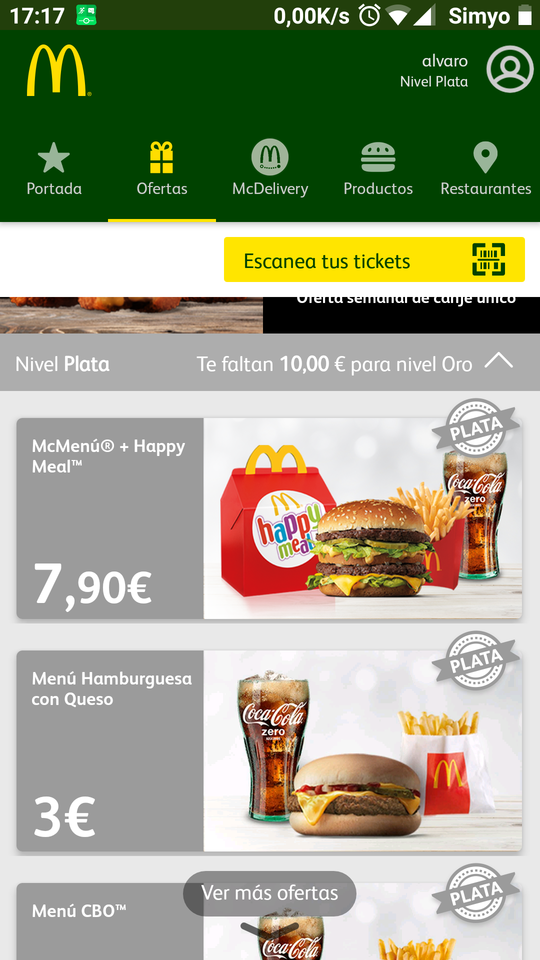
\includegraphics[scale=0.25]{images/restaurantes/mcdo0.png}
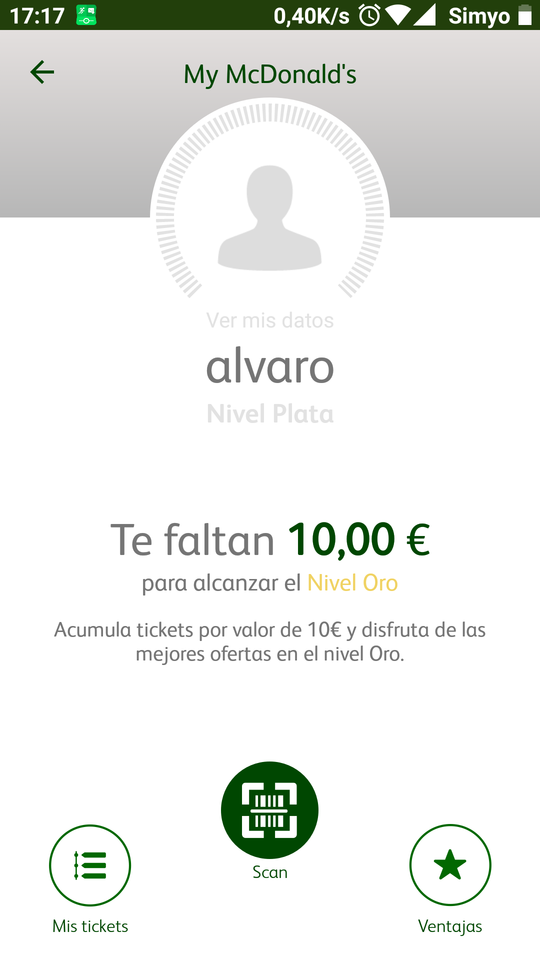
\includegraphics[scale=0.25]{images/restaurantes/mcdo1.png}
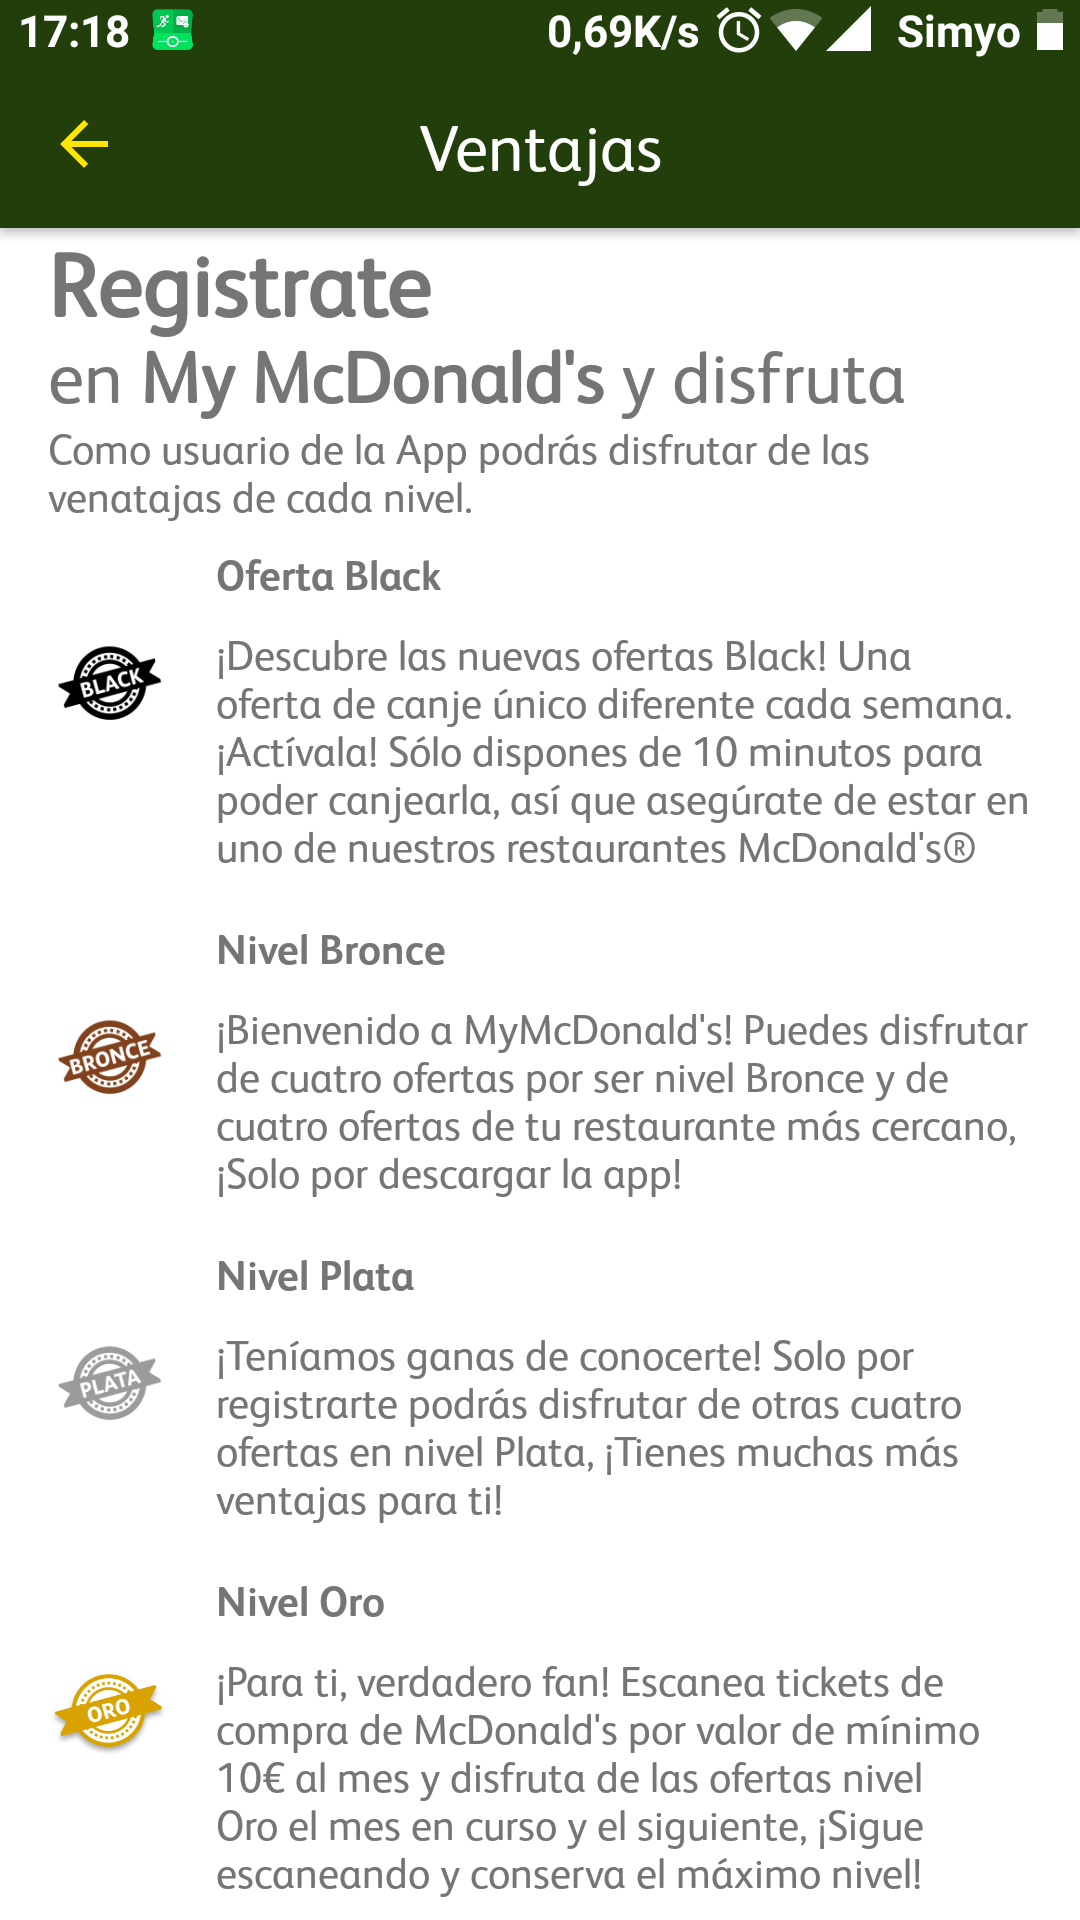
\includegraphics[scale=0.25]{images/restaurantes/mcdo3.png}
\caption{Capturas de pantalla de la aplicación \textit{"McDonald's España - Ofertas"}.} \cite{mcdo}
\end{center}
\end{figure}

\begin{itemize}
\item \textbf{Aplicación estudiada:} \cite{mcdo} \textit{McDonald's España - Ofertas.}
\item \textbf{Análisis:} 
La aplicación móvil McDonalds ofrece un gran número de funcionalidades, entre las que se encuentran un servicio de ofertas , canjeo de cupones, listado de la carta de productos o envío de pedidos a domicilio. 

No tiene un sistema de ludificación implementado, ya que su estrategia se basa en utilizar un sistema por niveles (oro, plata y bronce), en el que cuanto más alto sea, mejores ofertas se pueden encontrar. Para poder subir de nivel, será necesario escanear los tickets de compra y llegar a un mínimo de gasto.

Destacar que durante el tiempo que ha estado instalada ha pedido dar la opinión de la app por correo electrónico, a cambio de obtener un obsequio.
\item \textbf{Puntos fuertes:}
	\begin{itemize}
	\item Promueve el consumo de los clientes en los restaurantes de la cadena, recomendándoles hacer un determinado gasto para poder mantenerse en el mismo nivel.
	\item Ofertas \textit{"Black"}: Son ofertas que se activan solo durante diez minutos y hay que estar presente en el local en ese momento para canjearla.
	\end{itemize}
\item \textbf{Puntos débiles:}
	\begin{itemize}
	\item Se limita al consumo y no a promocionar la marca por redes sociales, gracias a la ayuda de los clientes.
	\item Las promociones solo se pueden hacer efectivas en los establecimientos físicos, no en pedidos por Internet.
	\item No existe ningún historial de pedidos.
	\end{itemize}
\end{itemize}


\subsubsection{Burger King}

\begin{figure}[H]
\begin{center}
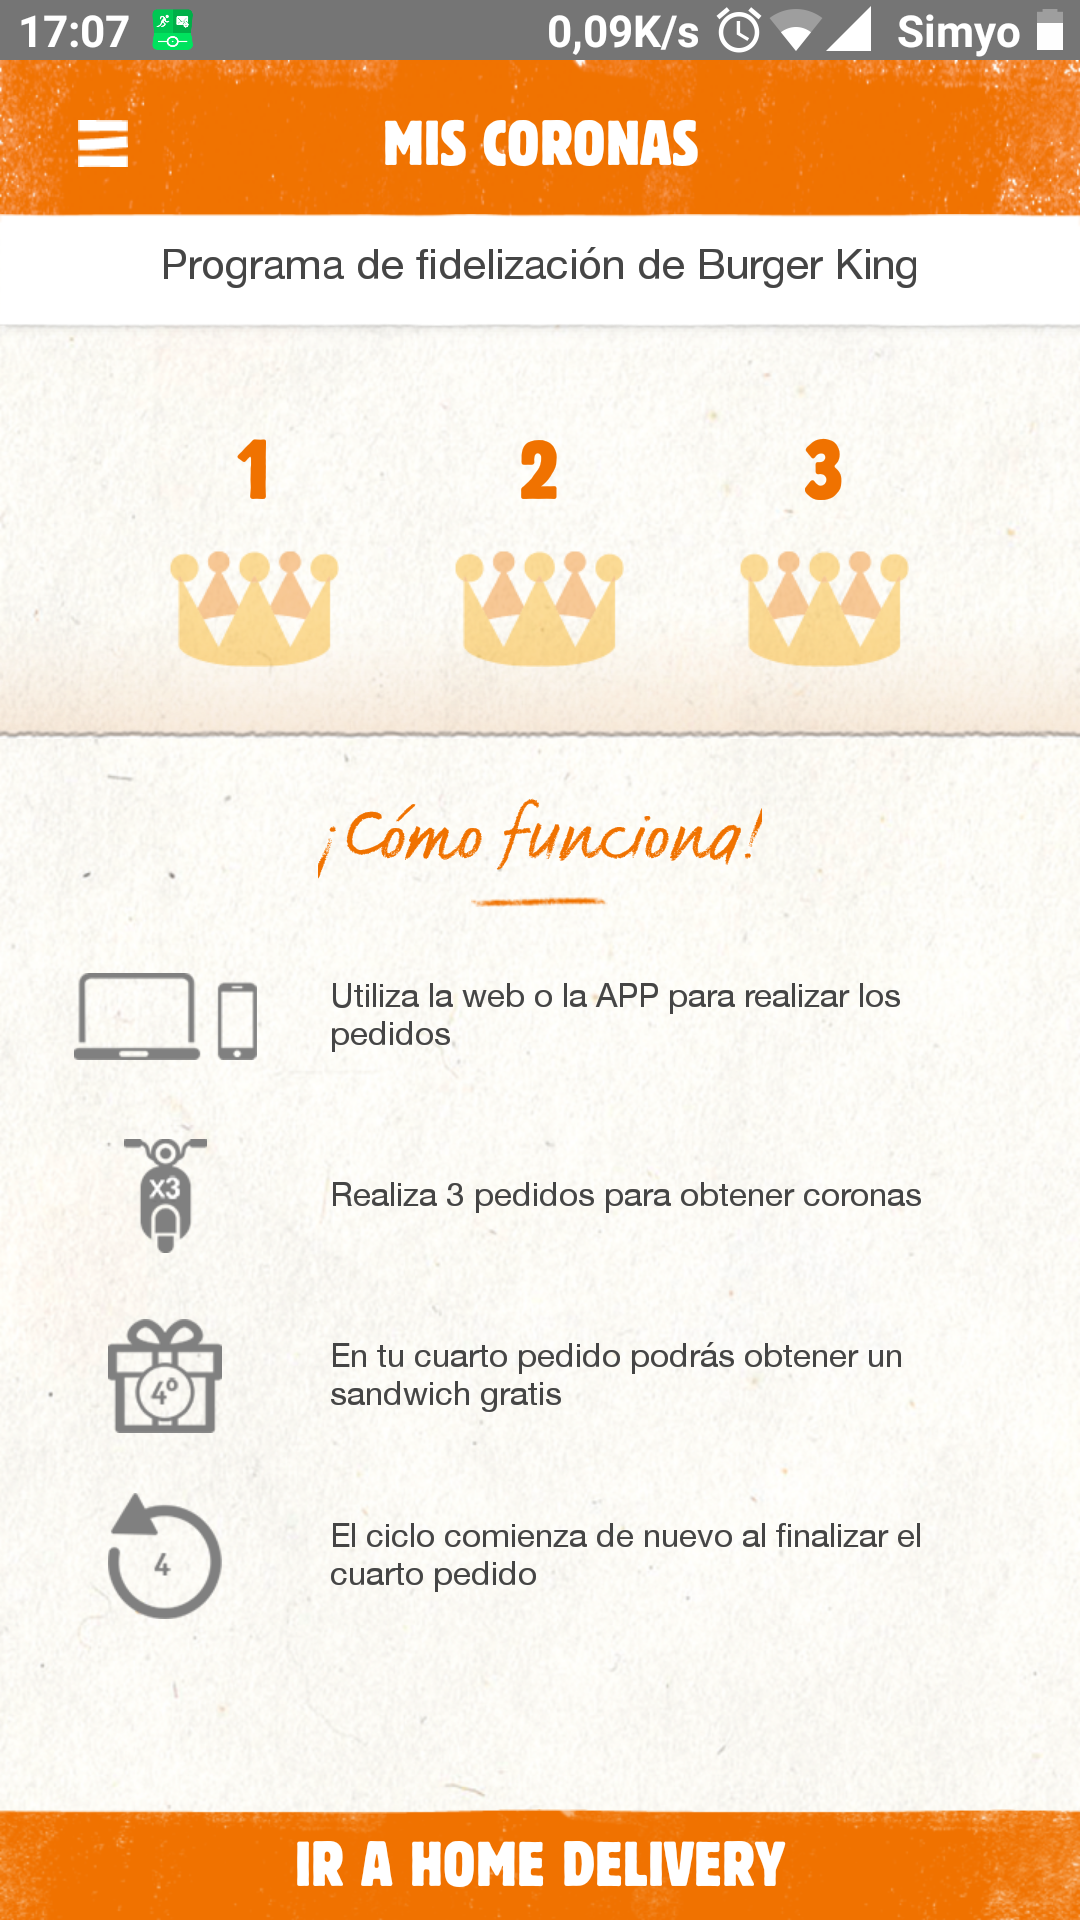
\includegraphics[scale=0.25]{images/restaurantes/burry0.png}
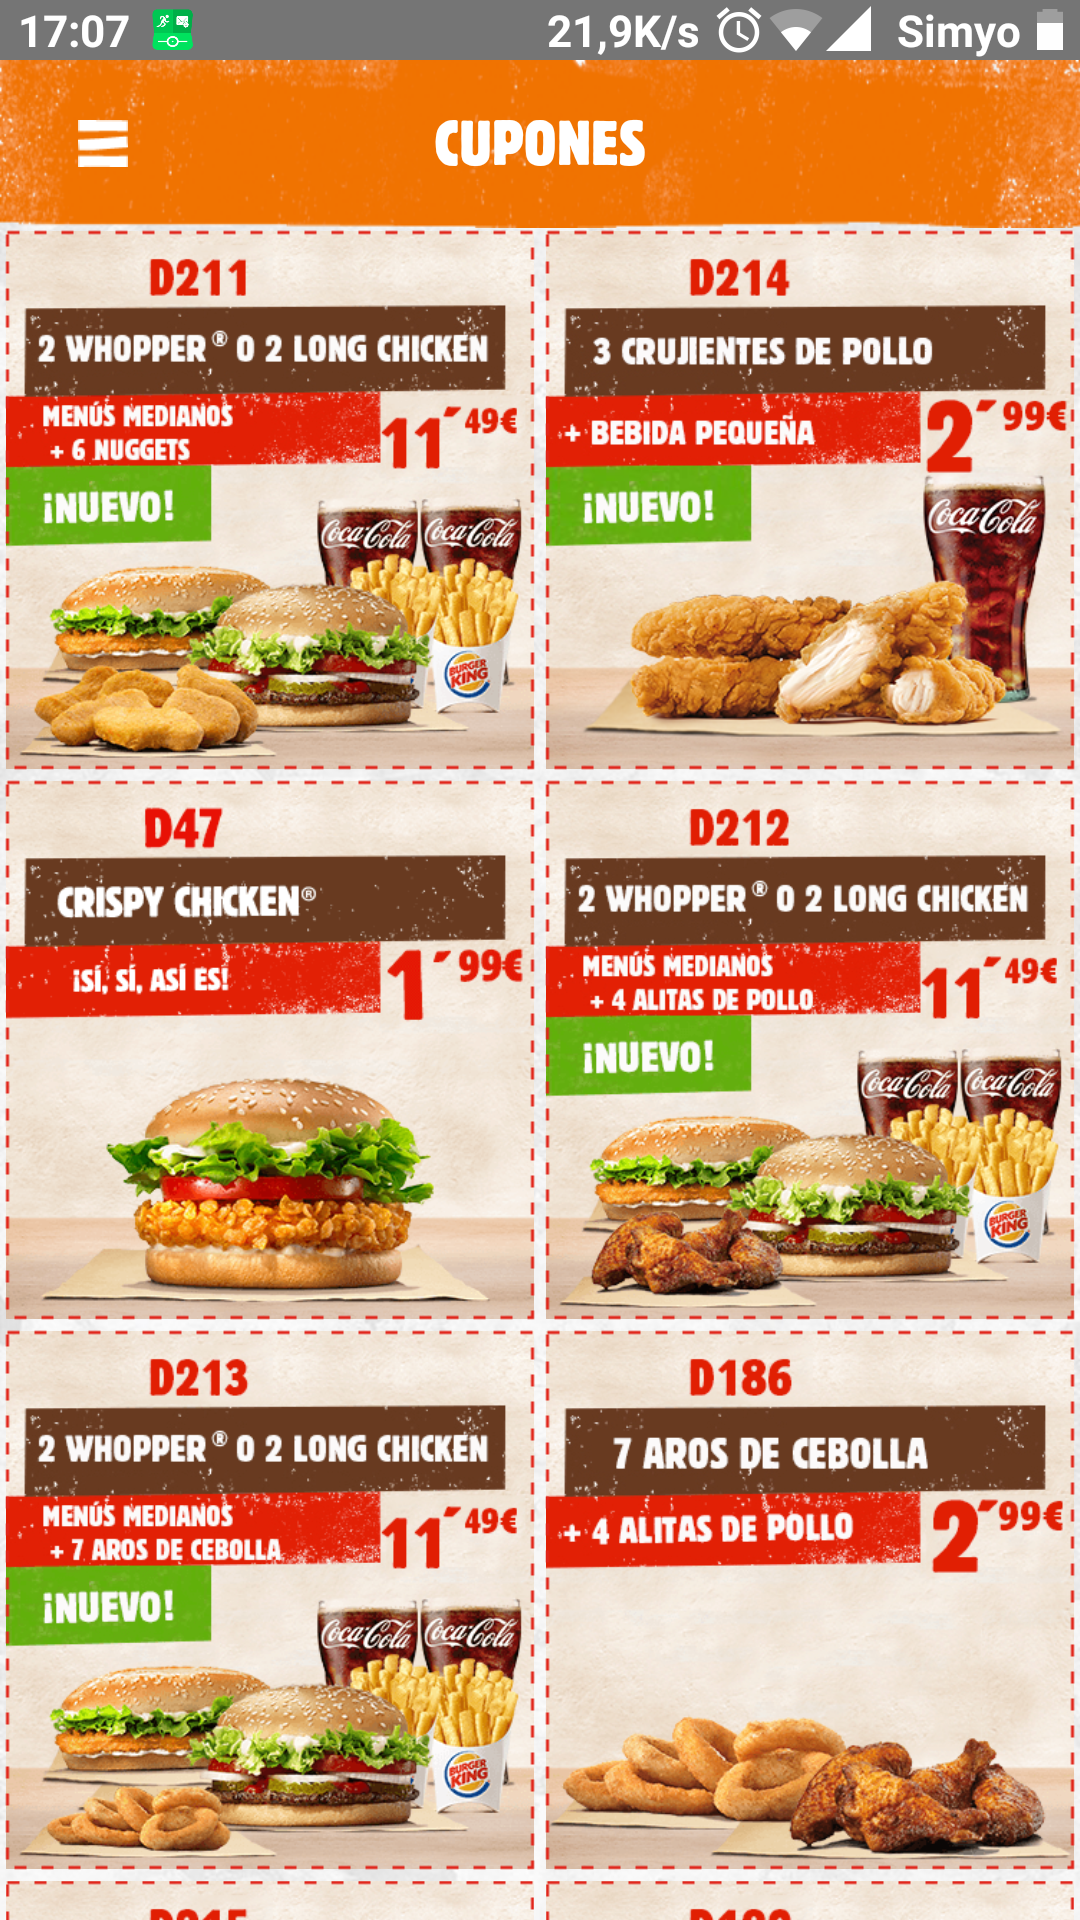
\includegraphics[scale=0.25]{images/restaurantes/burry1.png}
\caption{Capturas de pantalla de la aplicación \textit{"BURGER KING® España"}.} \cite{burgerk}
\end{center}
\end{figure}

\begin{itemize}
\item \textbf{Aplicación estudiada:} \cite{burgerk} \textit{BURGER KING® España.}
\item \textbf{Análisis:} 
Al igual que McDonalds, sí se ofrece un sistema de fidelización, llamado "Mis Coronas". Este programa consiste en que cada tres pedidos realizados por medio de la app móvil o el sitio web de Burger King se acumulan coronas. Cada cuatro coronas se consigue una hamburguesa gratis. Además, invitan a registrarse en la app, ya que, con el historial de pedidos realizarán ofertas personalizadas al cliente.

Las opciones de esta app están bastante limitadas y en ellas se encuentran conseguir un listado de restaurantes, realizar pedidos a domicilio, ver la carta de productos o visualizar un listado de cupones o promociones.
\item \textbf{Puntos fuertes:}
	\begin{itemize}
	\item Avisa mediante notificaciones \textit{PUSH} de nuevas ofertas.
	\item Solicita seguir a la marca por redes sociales (\textit{Facebook}).
	\item Tiene un sistema de fidelización para sus pedidos \textit{online}.
	\item Permite visualizar el historial de pedidos por Internet.
	\end{itemize}
\item \textbf{Puntos débiles:}
	\begin{itemize}
		\item La parte de fidelización está solo dedicada a la realización de pedidos por Internet.
		\item Las promociones son muy similares, independientemente del perfil del cliente.
		\item No está orientada a que el cliente realice un determinado consumo.
		\item No se pueden aplicar los cupones de la aplicación a pedidos a domicilio.
	\end{itemize}
\end{itemize}

\subsubsection{KFC}

\begin{figure}[H]
\begin{center}

\includegraphics[scale=0.25]{images/restaurantes/kfc0.png}
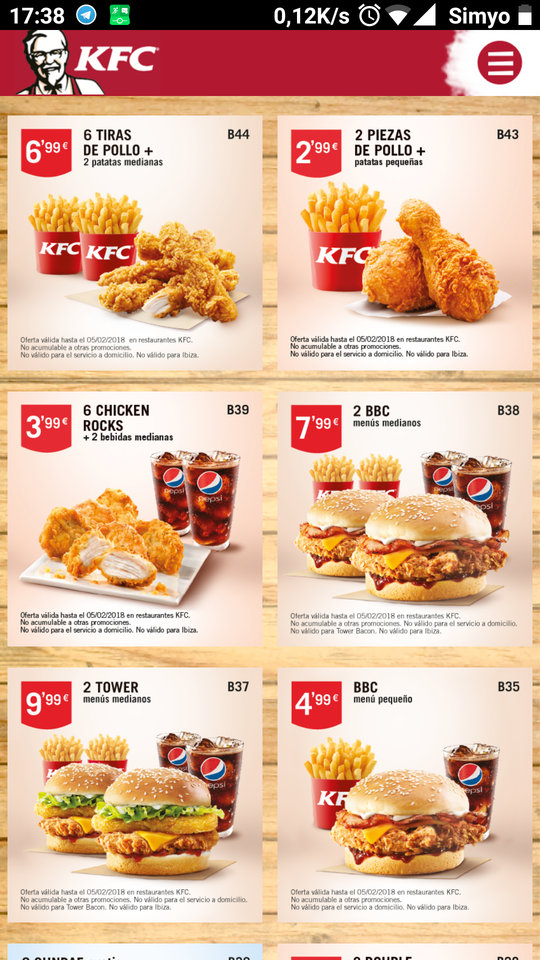
\includegraphics[scale=0.25]{images/restaurantes/kfc1.png}
\caption{Capturas de pantalla de la aplicación \textit{"KFC España–ofertas cerca de ti"}.} \cite{kfcapp}
\end{center}
\end{figure}


\begin{itemize}
\item \textbf{Aplicación estudiada:} \cite{kfcapp} \textit{KFC España–ofertas cerca de ti.}
\item \textbf{Análisis:} 

Es una de las aplicaciones más básicas de las estudiadas pues se limita a poner una carta de productos, un listado de restuarantes y una opción para obtener ofertas.

\item \textbf{Puntos fuertes:}
	\begin{itemize}
	\item Notificaciones \textit{PUSH} para notificar al cliente de nuevas ofertas y promociones.
	\end{itemize}
\item \textbf{Puntos débiles:}
	\begin{itemize}
	\item No tiene un sistema de fidelización.
	\end{itemize}
\end{itemize}

\subsubsection{VIPS}

\begin{figure}[H]
\begin{center}

\includegraphics[scale=0.25]{images/restaurantes/vips0.png}

\includegraphics[scale=0.25]{images/restaurantes/vips1.png}

\includegraphics[scale=0.25]{images/restaurantes/vips2.png}
\caption{Capturas de pantalla de la aplicación \textit{“Club VIPS: Promociones y pedidos Take Away"}.} \cite{vipsapp}
\end{center}
\end{figure}

\begin{itemize}
\item \textbf{Aplicación estudiada:} \cite{vipsapp} \textit{Club VIPS: Promociones y pedidos Take Away.}
\item \textbf{Análisis:} 
La aplicación de la cadena VIPS es, sin lugar a dudas, la más completa de las analizadas.

Para fidelizar clientes, utiliza el servicio ClubEuroVIPS, en el que ofrece un \textit{cashback} de un 3\%, pudiendo duplicarse bajo ciertas condiciones. Además ofrece un sistema de clasificación de usuarios según su consumo (niveles clásico, oro y platino), en el que, dependiendo del cuál nos escontremos podremos obtener \textit{WiFi} Premium, bebidas extras u obtener puntos extras.

Paralelamente, la aplicación invita al usuario, con cierta frecuencia a sus lanzamientos o estrenos de nuevos productos. Por ejemplo “\textit{te invitamos a nuestras hamburguesas del Chef o a nuestras nuevas pizzas Chicago Style}” o “\textit{te invitamos a probar nuestras pizzas}”.

Similarmente, se pueden encontrar funcionalidades propias de un restaurante que apuesta por el crecimiento de su app móvil, como son la posibilidad de pagar un pedido con la app móvil, la funcionalidad \textit{Shake-It}, que consiste en realizar tu pedido favorito con solo agitar tu teléfono móvil o la posibilidad de guardar promociones en la aplicación. Además, también permite realizar pedidos online del tipo \textit{take-away}.
\item \textbf{Puntos fuertes:}
	\begin{itemize}
	\item La aplicación integra la tarjeta \textit{Club VIPS}, que permite sumar puntos gracias a las compras hechas en restaurantes de la marca.
	\item Se puede duplicar el valor de los puntos del  \textit{Club VIPS} bajo ciertas circunstancias ligadas a un mayor consumo o a ciertas franjas horarias.
	\item Notificaciones \textit{PUSH} para notificar al cliente de nuevas ofertas y promociones.
	\item Cuenta con un historial de pedidos.
	\item Integra un sistema para conectarse automáticamente con las redes \textit{WiFi} de los restaurantes de la marca. Posibilidad de tener \textit{WiFi} Premium en caso de alcanzar un cierto consumo.
	\item Permite capturar nuevas promociones escaneando el código \textit{QR} de la publicidad.
	\item Invitaciones a eventos por el hecho de ser usuario de un determinado nivel.
	\item Existe un conjunto de niveles, determinados por el consumo que se hace en los restaurantes.
	\item Se realiza \textit{cashback} en los pedidos realizados siendo socio del \textit{Club VIPS}.
	\item Se puede conseguir hasta un 25\% de descuento al invitar a usuarios a hacerse socios del \textit{Club VIPS}.
	\end{itemize}
\item \textbf{Puntos débiles:}
	\begin{itemize}
	\item No existe ningún juego ni interacción con redes sociales.
	\end{itemize}
\end{itemize}

\subsubsection{Pans \& Company}

\begin{figure}[H]
\begin{center}

\includegraphics[scale=0.25]{images/restaurantes/pans0.png}

\includegraphics[scale=0.25]{images/restaurantes/pans1.png}
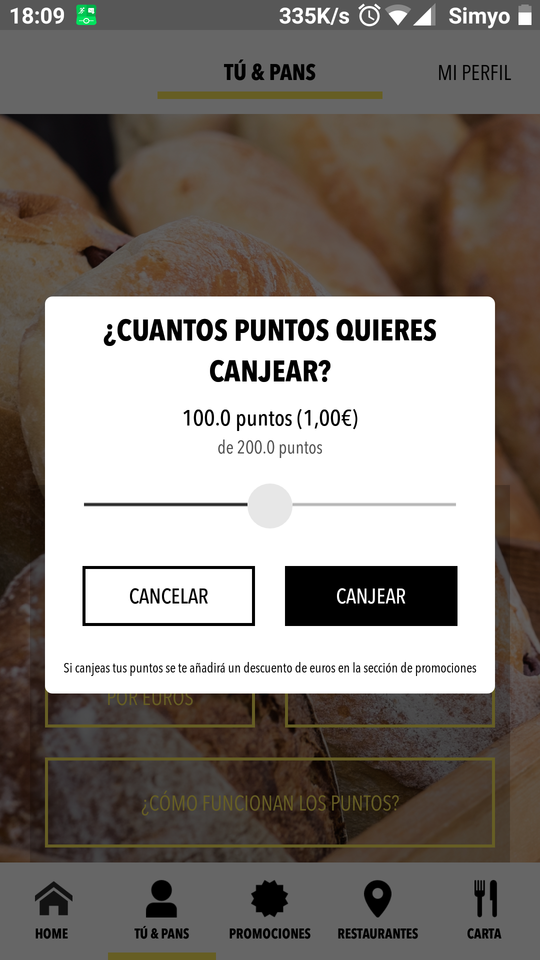
\includegraphics[scale=0.25]{images/restaurantes/pans2.png}
\caption{Capturas de pantalla de la aplicación \textit{"Pans \& Company"}.} \cite{pansapp}
\end{center}
\end{figure}

\begin{itemize}
\item \textbf{Aplicación estudiada:} \cite{pansapp} \textit{Pans \& Company.}
\item \textbf{Análisis:} 
Pans \& Company ofrece únicamente una tarjeta de fidelidad, integrada en la misma app. Esta tarjeta básicamente consiste en un código QR que el usuario puede mostrar en caja para acumular puntos que, posteriormente se podrán convertir en dinero. Además, se realizarán ofertas personalizadas.

Sus funcionalidades son las típicas de una aplicación de esta categoría: listado de restaurantes, ofertas y listado de la carta.
\item \textbf{Puntos fuertes:}
	\begin{itemize}
	\item Notificaciones \textit{PUSH} para notificar al cliente de nuevas ofertas y promociones.
	\item La aplicación integra una tarjeta de fidelización en el que se acumulan puntos a la hora de realizar compras. Los puntos se podrán canjear posteriormente por descuentos en compras en los restaurantes.
	\end{itemize}
\item \textbf{Puntos débiles:}
	\begin{itemize}
	\item No cuenta con interacción entre usuarios ni redes sociales, se limita a la tarjeta de fidelización.
	\end{itemize}
\end{itemize}

\subsubsection{Foster's Hollywood}

\begin{figure}[H]
\begin{center}

\includegraphics[scale=0.25]{images/restaurantes/foster0.png}

\includegraphics[scale=0.25]{images/restaurantes/foster1.png}
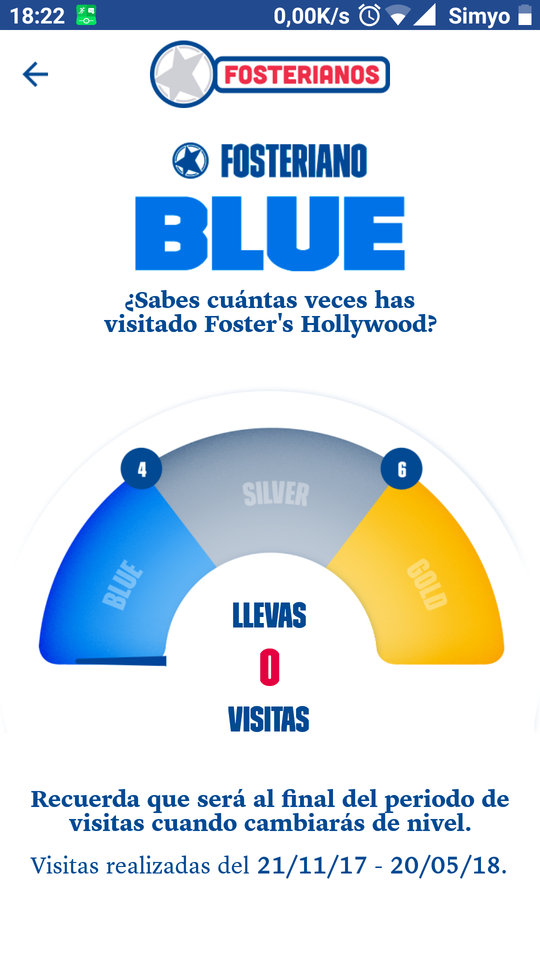
\includegraphics[scale=0.25]{images/restaurantes/foster2.png}
\caption{Capturas de pantalla de la aplicación \textit{"Foster's Hollywood"}.} \cite{fostersh}
\end{center}
\end{figure}

\begin{itemize}
\item \textbf{Aplicación estudiada:} \cite{fostersh} \textit{Foster's Hollywood.}
\item \textbf{Análisis:} 
El sistema de fidelización de clientes de Foster's Hollywood se basa en un sistema de niveles (\textit{blue}, \textit{silver} y \textit{gold}), en el que cuanto mejor sea el nivel, mayores ventajas tendrá el usuario, entre las que se encuentran un postre de regalo, descuentos de ocio (en empresas asociadas), o incluso, promoción por el cumpleaños. Para poder aumentar de nivel será necesario ir un número de veces a los establecimientos de la cadena. 

Se nos identificará como clientes mediante la tarjeta Foster's Hollywood, que consiste en un código QR localizado en la aplicación y que el cliente simplemente debe enseñar al realizar el pago, con el fin de que la compra quede asociada a su usuario.

Por otra parte, también es posible visualizar la carta del restaurante o ver el listado de restaurantes, así como realizar el pedido online.
\item \textbf{Puntos fuertes:}
	\begin{itemize}
	\item Notificaciones \textit{PUSH} para notificar al cliente de nuevas ofertas y promociones.
	\item Sistema de fidelización basado en niveles e integrado en la aplicación.
	\end{itemize}
\item \textbf{Puntos débiles:}
	\begin{itemize}
	\item No cuenta con interacción entre usuarios ni redes sociales, se limita al sistema de fidelización.
	\end{itemize}
\end{itemize}

\subsection{Conclusiones extraídas}

Extraigo las siguientes conclusiones a partir de las aplicaciones móviles analizadas:
\begin{itemize}
\item Ninguna emplea un sistema de gamificación.
\item Los sistemas de fidelización de clientes son bastante limitados, siendo, en muchos casos, una simple tarjeta virtual donde acumular puntos.
\item Todas ofrecen un sistema para obtener ofertas.
\item Las aplicaciones se limitan a la interacción Usuario-Empresa, ninguna emplea las redes sociales para aumentar su base de usuarios.
\item La mayoría de las aplicaciones (todas exceptuando Burger King y KFC) promueven que el usuario vuelva al local, mediante la realización de ofertas específicas para ello.
\end{itemize}

\section{Estructura de la memoria}

Este documento está divido en partes y a su vez estas en secciones y subsecciones, abarcando así los distintos documentos recogidos en esta memoria:

\begin{itemize}
\item Parte I. Introducción y Objetivos: incluye una breve explicación de lo que es la ludificación, así como una explicación a alto nivel de la propuesta realizada por la diseñadora del sistema de ludificación sobre el que está basado el proyecto. Finalmente, también contiene un análisis de aplicaciones de restaurantes de comida rápida que operan en España, con el fin de estudiar si estos incluyen o no un sistema de ludificación.

\item Parte II. Herramientas utilizadas: detallaré aquellas herramientas utilizadas en el proyecto, tanto de tipo \textit{hardware} como de tipo \textit{software}. 

\item Parte III. Route66App: es la parte más importante del proyecto, pues incluye la gran mayoría de documentos, como el Plan de Desarrollo de Software, el documento de análisis, el documento de diseño, los prototipos realizados y todos aquellos detalles de la implementación que merece la pena reseñar.

\item Parte IV. Conclusiones y líneas futuras.

\item Referencias.

\item Anexos

\end{itemize}

\section{Propuesta.}
Este Trabajo de Fin de Grado estará centrado en el TFG “Estudio de ludificación en una empresa para mejorar la fidelización de los clientes”\cite{cristinatfg}, elaborado por Dª Cristina Martínez Martínez, graduada durante el curso 2016-2017 en Ingeniería de Organización Industrial por la Universidad de Valladolid.  

El trabajo de esta alumna, centrado en el diseño de un sistema de ludificación aplicado a un posible caso real (restaurante de comida americana), tenía el problema de la imposibilidad de llevarlo a cabo con herramientas profesionales, debido a su coste y a la falta de disponibilidad de las mismas. Por este motivo, el TFG se tuvo que defender contando solo con una serie de prototipos basados en un sistema web. 

Como la ludificación es un área en investigacion y que ofrece muy buenos resultados, la tutora del TFG propuso a la Comisión de Título la realización de este trabajo. Por otro lado, el resultado del mismo puede servir a alumnos de otras facultades para poder utilizar una herramienta de ludificación real.

\subsection{Resumen de “Estudio de ludificación en una empresa para mejorar la fidelización de los clientes”}

Se propone la realización de un sistema de ludificación para una cadena de restaurantes de comida americana, que cuenta con un conjunto de franquicias repartidas por todo el territorio español. Es una empresa con muy buenos resultados económicos y cuenta con una amplia y sólida base de clientes, que decide elaborar una aplicación que mejore la opinión de los mismos sobre la marca, ya que han llegado críticas sobre el sistema vigente de cupones y descuentos.

Finalmente, el equipo directivo decide encargar una aplicación basada en la ludificación cuyos objetivos son los siguientes:

\begin{enumerate}
\item Aumentar la fidelización de los clientes.
\item Incentivar las ventas.
\item Mejorar la imagen de la marca en redes sociales.
\item Conseguir nuevos clientes.
\item Mejorar la confianza y satisfacción del cliente. 
\end{enumerate}

Se medirá el cumplimiento de los objetivos anteriores mediante el cálculo de una serie de ratios.\\

\textbf{Público objetivo}\\

El público objetivo estará formado por hombres y mujeres, cuyas edades estén comprendidas entre los doce y los cincuenta y cinco años. 
Los conocimientos tecnológicos esperados en este grupo de edad no tienen por qué ser altos, ya que se utilizará una aplicación móvil. Se considerará suficiente por tanto, conocimientos básicos en uso de smartphones y de uso de aplicaciones móviles. En el caso en el que nos encontramos la aplicación a desarrollar será Android.

Los potenciales usuarios de la aplicación la utilizarán para conseguir recompensas y descuentos derivados del uso de la misma.

Finalmente, indicar que se clasificará cada jugador en función de sus gustos y comportamientos, siguiendo la teoría de Battle, haciendo así que la experiencia de usuario sea distinta entre usuarios de distinta categoría. En concreto, se realizarán distintos tipos de juegos.\\

\textbf{Roles}\\

Se proponen dos tipos de roles: Administrador y Cliente.

Las funcionalidades que podrá acceder cada tipo de rol vendrán determinadas en un diagrama de casos de uso que se especificará en el apartado correspondiente. \\

\textbf{Descripción del juego}\\

El juego se centra en un mapa de la Ruta66 americana, aprovechando así la temática del restaurante. Se dividirá el camino en once etapas o niveles, correspondientes a las principales ciudades por las que pasa esta vía, y para avanzar, el cliente deberá completar una serie de actividades, que además otorgarán insignias. Cabe destacar que la dificultad de los niveles irá aumentando gradualmente, con el objetivo de no perder la motivación.

\begin{multicols}{4}
\begin{enumerate}
\item Chicago.
\item Springfield.
\item St. Louis.
\item Tulsa.
\item Oklahoma City.
\item Amarillo.
\item Santa Fe.
\item Albuquerque.
\item Flagstaff.
\item Williams.
\item Los Ángeles.
\end{enumerate}
\end{multicols}

Todos los niveles excepto el de Chicago tendrán un planteamiento similar:
\begin{itemize}
\item Nivel 1. Chicago: Compuesto por diez casillas. Se activarán dos por cada actividad completada:
	\begin{itemize}
		\item Configuración del perfil del jugador.
		\item Crear un equipo.
		\item Seguir en redes sociales la página del restaurante.
		\item Puntuar la aplicación en la tienda de aplicaciones.
		\item Comentar la aplicación en la tienda de aplicaciones.
	\end{itemize}
\item Resto de niveles: Consistirán en diez misiones:
	\begin{itemize}
		\item Misiones de nivel social: consistirán en tareas como compartir el progreso, subir una foto hecha en el restaurante a las redes sociales, enviar invitaciones…
		\item Misiones de minijuegos: serán dos casillas y consistirá en jugar a un minijuego, dependiente del perfil de jugador.
		\item Misiones de consumo: el jugador deberá realizar consumiciones en los restaurantes de la cadena. Avanzará más o menos casillas en función del gasto que realice.
		\item Misiones de retos especiales: en días señalados, los jugadores podrán participar en retos creados específicamente para ese día.
	\end{itemize}
\end{itemize}

\textbf{Recompensas}\\

Hay tres tipos de recompensa:
\begin{itemize}
\item Puntos: el usuario obtendrá diez puntos por cada casilla que avance. Similarmente, se agrupará la suma total en tres categorías: consumo, social y competitivo.
\item Insignias: cuando el jugador haya completado un nivel completo obtendrá una insignia (matrícula de la ciudad asociada). Habrá, adicionalmente, otras insignias, entre las que se encuentran la familiar o las de grupo.
\item Premios: los premios serán regalos. Se desbloquearán cuando el usuario haya completado un nivel o haya realizado algún reto especial.
\end{itemize}

\textbf{Perfiles de jugador\cite{iebsctj}}\\ 

Todos los jugadores tendrán asociado un perfil, que se determinará en el registro de usuario:
\begin{itemize}

\item Triunfador: tendrá como objetivo llevar a cabo las misiones y obtener los premios o recompensas.
\item Explorador: son jugadores que les gusta descubrir o aprender cosas nuevas.
\item Socializadores: más que interés en conseguir los logros, buscan aprovecharlos para entablar relaciones sociales.
\item Killers: buscan ser los primeros en el juego. Quieren destacar sobre otros jugadores.

\end{itemize}

\textbf{Grupos}\\

Los jugadores, similarmente, podrán crear el número que quieran de equipos. Participarán con los mismos a la hora de alcanzar las recompensas.

\chapter{Parte II: Herramientas utilizadas}
\section{Herramientas utilizadas}

Para la elaboración de esta memoria he utilizado las siguientes herramientas:
\begin{itemize}
\item Como editor \LaTeX , Texmaker v. 4.4.1. \footnote{\url{http://www.xm1math.net/texmaker/}}
\item Como sistema de control de versiones, GitHub \footnote{\url{https://www.github.com}}
\item Para la realización de backups, Dropbox \footnote{\url{https://www.dropbox.com/}}
\item Para tomar notas e ideas, Dropbox Paper \footnote{\url{https://paper.dropbox.com}}
\item Para realizar los diagramas \textit{UML}, Astah Professional 7.1.0  \footnote{\url{http://astah.net/}}
\end{itemize}

Para la elaboración de los prototipos, he utilizado Ionic 3 \footnote{\url{https://ionicframework.com/}}.

Para la elaboración de la aplicación Android, he utilizando Android Studio.

Para el control y seguimiento del proyecto utilizaré la herramienta Zoho Projects \footnote{\url{https://projects.zoho.com/}}.

Finalmente, he empleado Firebase \footnote{\url{https://firebase.google.com/}}

\section{Comunicación con el servidor}

\chapter{Parte III: Route66App}
\section{Plan de Desarrollo del Software}
\subsection{Descripción del proyecto}
La ludificación comenzó a popularizarse en 2010\cite{anatfg}. Desde entonces, tal y como he explicado en puntos anteriores de esta memoria, se ha aplicado en numerosas situaciones (educación, ventas, proveedores, etcétera). En el caso que nos ocupa, un restaurante de comida americana, no podemos encontrar en España ningún ejemplo de una aplicación similar que aplique la ludificación.

Route66App consiste en una app para dispositivos móviles que aplica las ideas expuestas en el Trabajo Fin de Grado de una alumna del Grado en Organización Industrial \cite{cristinatfg}. Esta aplicación aplicará la teoría Bartle para identificar los diferentes tipos de jugador y buscará fidelizar y comprometer al usuario con los objetivos del negocio, por medio del juego.

Es importante destacar que este trabajo es solo una parte de dos, el cliente. Para un completo funcionamiento se requerirá el gestor web, en el que se podrán añadir y modificar las diferentes misiones que conforman el juego.
 
\subsubsection{Propósito, objetivos y alcance}

El objetivo fundamental de  este trabajo es el de la implementación de un sistema de ludificación, aplicado a un restaurante de comida americana. En concreto se realizará la parte cliente, ejecutada desde terminales móviles con el Sistema Operativo Android.

La aplicación deberá contar con las siguientes funciones:
\begin{itemize}
\item Acciones propias del usuario
	\begin{itemize}
	\item Realizar misiones y juegos, con el fin de conseguir puntos y aumentar el nivel o posición en un ranking.
	\item Modificación del perfil del usuario, permitiendo actualizar el avatar del usuario.
	\item Consulta del historial de logros del usuario.
	\item Consulta de las insignias del usuario.
	\item Consulta del código QR que identifica al usuario de forma única.
	\item Consulta de la posición global del usuario (ranking).
	\end{itemize}
\item Acciones a realizar en grupo.
	\begin{itemize}
	\item Cosulta de los equipos a los que pertenece el usuario.
	\item Creación de nuevos equipos.
	\end{itemize}
\end{itemize}

Los objetivos serán:
\begin{itemize}
	\item Elaborar un sistema de usuarios, mediante el uso de sesiones.
	\item Gestionar un sistema de insignias, otorgadas tanto a usuarios individuales, como a grupos o equipos completos.
	\item Aumentar el compromiso del usuario con la aplicación, mediante el uso de juegos o misiones. Se busca que el usuario realice acciones correspondientes a los cuatro roles mencionados anteriormente.
	\item Hacer las funciones de una tarjeta de fidelización virtual, que permita al usuario identificarse a la hora de pagar.
\end{itemize}

\subsection{Metodología de Desarrollo del proyecto}
El proyecto aplicará el Proceso Unificado (\textit{Unified Process}), en concreto el proceso UPedu \cite{upedu}, cuyas caracterísiticas básicas \cite{pgpup} son: 
\begin{itemize}
\item Dirigido por los casos de uso.
\item Centrado en la arquitectura.
\item Iterativo e incremental
\end{itemize}
La iteratividad supone ciertas ventajas, como que se pueden mitigar los riesgos más críticos en las fases más tempranas o que permite obtener \textit{feedback} mucho antes, además, el aprendizaje obtenido se puede reaprovechar en etapas posteriores.

\subsection{Restricciones}
Se imponen las siguientes restricciones:
\begin{enumerate}
\item \textbf{Tiempo:} Este proyecto se realiza para cumplir con los objetivos de la asignatura Trabajo de Fin de Grado. Mención Ingeniería del Software, correspondiente a 12 créditos ECTS, unas 300 horas.

\item \textbf{Plazo mínimo de entrega:} Este proyecto se podrá entregar cuando haya terminado el resto de asignaturas de la Mención. Por tanto, hasta que no termine y tenga calificada la única asignatura que tendré en el segundo cuatrimestre (Prácticas de Empresa), no podrá ser entregado. Las prácticas curriculares en la empresa \textit{Telefónica Investigación y Desarrollo} concluyen el día 10 de Abril de 2018.

\item \textbf{Requisitos de la plataforma:} La aplicación será instalable en terminales Android, cuya versión de API sea igual o superior a la 19 (Android 4.4, KitKat). Según el sitio Web oficial de desarrolladores de Android \footnote{\url{https://developer.android.com/}}, esto supone cubrir la grandísima mayoría de los dispositivos (un 92.5, a fecha 25 de Noviembre de 2017)\cite{androidversiondist}.

\item \textbf{Persistencia de datos: } Contaré con el servicio de gestión de bases de datos SQLite que ofrece Android de serie, con el fin de reducir la carga de peticiones que haga el usuario contra la plataforma.
\end{enumerate}

\subsection{Estructura organizativa}
\subsubsection{Estructura organizativa interna}
La estructura organizativa del proyecto estará formada por una única persona, que deberá ejercer cada uno de los roles en el momento en el que sea necesario. \cite{upedu} \vspace{0.5cm}

\begin{table}[H]
\begin{tabular}{llll}
\cline{1-2}
\multicolumn{1}{|c|}{Rol} & \multicolumn{1}{c|}{Encargado} &  &  \\ \cline{1-2}
\multicolumn{1}{|l|}{Desarrollador}                                      & \multicolumn{1}{l|}{Álvaro Carreras}                                          &  &  \\ \cline{1-2}
\multicolumn{1}{|l|}{Analista}                                           & \multicolumn{1}{l|}{Álvaro Carreras}                                          &  &  \\ \cline{1-2}
\multicolumn{1}{|l|}{Gestor de proyecto}                                 & \multicolumn{1}{l|}{Álvaro Carreras}                                          &  &  \\ \cline{1-2}
\multicolumn{1}{|l|}{Diseñador}                                          & \multicolumn{1}{l|}{Álvaro Carreras}                                                         &  &  \\ \cline{1-2}
                                                                         &                                                                               &  & 
\end{tabular}
\centering
\caption{Roles}
\end{table}
\vspace{0.5cm}

\paragraph{Desarrollador}\mbox{}\\

Este rol se encarga de implementar el código y de realizar las pruebas para los entregables software generados, con el fin de que sean integrados.

\paragraph{Analista}\mbox{}\\

Organiza y coordina tanto la elicitación de requisitos como el modelado de casos de uso indicando y limitando la funcionalidad del sistema y el alcance del mismo.

\paragraph{Gestor de Proyecto}\mbox{}\\

Realiza el control y mando del proyecto, asigna recursos, gestiona los reisgos, distribuye responsabilidades, gestiona la interacción con los clientes, etcétera.

\paragraph{Diseñador}\mbox{}\\

Como indica su nombre, está encargado de diseñar el sistema, definiendo las responsabilidades, operaciones y relaciones de cada uno de los componentes del sistema.

\subsubsection{Estructura organizativa externa}
Solo se identifica un rol en la estructura organizativa externa: el del usuario de la aplicación. 

\subsection{Gestión del proyecto}
\subsubsection{Planificación del proyecto}
En este proyecto se utilizará la metodología UPedu \cite{upedu}, compuesta por fases y estas por iteraciones.

\begin{figure}[h]
\begin{center}
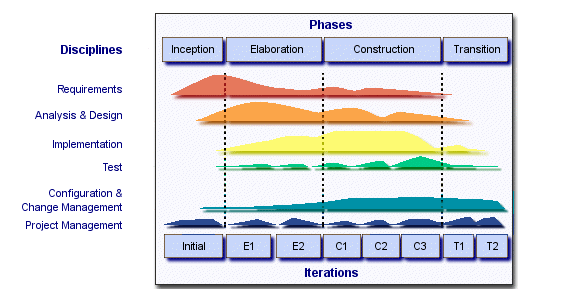
\includegraphics[scale=0.75]{images/upeduFases}
\caption{Fases de la metodología UPedu} \cite{upedu}
\end{center}
\end{figure}

En la figura anterior, se puede observar el esfuerzo necesario de cada disciplina en cada fase del proyecto

\paragraph{Fase de inicio}\mbox{}\\

En esta fase no se realiza ningún artefacto de tipo software, pues estos se deben tratar antes de comenzar con la implementación. Los objetivos fundamentales de esta fase son la definición del alcance del proyecto,  la determinación de los casos de uso críticos, la estimación del coste y la duración del proyecto, y la elaboración de una primera gestión de riesgos.

\paragraph{Fase de elaboración}\mbox{}\\

El objetivo fundamental de esta fase \cite{pgpup} es el de la elaboración del diseño y arquitectura del sistema informático. Similarmente, se realizará un análisis del dominio del sistema y se eliminarán los elementos de mayor riesgo para el desarrollo del proyecto.

Después de esta fase, se obtendrá una arquitectura, requisitos y planes de desarrollo estables. Similarmente, se habrán reducido los riesgos más destacables.

\paragraph{Fase de construcción}\mbox{}\\

Es sin ninguna duda la parte más larga del proyecto y es la primera que tendrá como output entregables software utilizables.Se irá iterando y mejorando la calidad del producto software en cada ciclo.

La salida de esta fase \cite{pgpup} es software en estado beta.

\paragraph{Fase de transición}\mbox{}\\

Se deberá conseguir la aceptación por parte del usuario, indicando que cumple con la visión inicial del proyecto. Asímismo, se distribuirá el software.

\subsubsection{Calendario del proyecto}

Como se ha indicado en los apartados anteriores, este proyecto se ha dividido en las fases que el Proceso Unificado, en su variación UPedu\cite{upedu} establece. A continuación, se lista cada fase, el número de iteraciones y las horas de trabajo y duración estimadas. Estos cálculos son orientativos, las variaciones sobre los mismos están expuestas en el apartado correspondiente.

\begin{table}[H]
\centering
\begin{tabular}{|l|l|l|l|}
\hline
Nombre de la fase & Núm.. Iteraciones & Horas de trabajo & Duración estimada \\ \hline
Inicio            & 1                 & 10 horas/semana  & 5 semanas       \\ \hline
Elaboración       & 2                 & 20 horas/semana  & 4 semanas     \\ \hline
Construcción      & 2                 & 20 horas/semana  & 6-7 semanas       \\ \hline
Transición        & 1                 & 5 horas/semana   & 2-3 semanas       \\ \hline
\end{tabular}
\caption{Fases del proceso UPedu}
\end{table}

\paragraph{Fase de inicio}\mbox{}\\

Comienza el día 6 de Noviembre de 2017 y finaliza el 10 de Diciembre de 2017. Consta de una única iteración. Solo trabajaré en el TFG durante los viernes y fines de semana.

\begin{table}[H]
\centering
	\begin{tabular}{|l|l|l|l|}
    \hline
    Nombre de la tarea                           & Fecha de comienzo & Fecha de fin & Duración \\ \hline
    Estudio del sistema.                         & 03/11/2017        & 05/11/2017   & 10 horas  \\ \hline
    Búsqueda de información.                     & 10/11/2017        & 11/11/2017   & 4 horas   \\ \hline
    Resumen de la propuesta                      & 11/11/2017        & 17/11/2017   & 6 horas   \\ \hline
    Estudio de aplicaciones móviles.             & 17/11/2017        & 17/11/2017   & 2 horas   \\ \hline
    Elaboración de un prototipo inicial          & 18/11/2017        & 19/11/2017   & 7 horas   \\ \hline
    Estudio de la posible tecnología a utilizar. & 19/11/2017        & 19/11/2017   & 3 horas   \\ \hline
    Plan de Desarrollo de Software.              & 24/11/2017        & 01/12/2017   & 13 horas   \\ \hline
    Elicitación de requisitos.                   & 01/12/2017        & 08/12/2017   & 12 horas   \\ \hline
    Identificación de riesgos.                   & 08/12/2017        & 09/12/2017   & 3 horas   \\ \hline
    Gestión de configuraciones.                  & 09/12/2017        & 10/12/2017   & 1 horas   \\ \hline
    \end{tabular}
    \caption{Iteración 0. Fase de Inicio.}
\end{table}

Reuniones realizadas con la tutora del TFG:

\begin{itemize}
\item 30 de Octubre de 2017.
\item 6 de Noviembre de 2017.
\item 20 de Noviembre de 2017.
\item 4 de Diciembre de 2017.
\end{itemize}

\paragraph{Fase de elaboración}\mbox{}\\

Decidí dejar un lapso temporal de 41 días (10 de Diciembre - 20 Enero) por la gran acumulación de trabajos y exámenes.

Esta fase comienza el día 20 de Enero de 2017 y finaliza el 1 de Marzo de 2018. Consta de dos iteraciones.

\begin{itemize}
\item Iteración 1: Con una duración de 3 semanas.
\item Iteración 2: Con una duración de 1 semana y media.
\end{itemize}

\begin{table}[H]
\centering
\begin{tabular}{|l|l|l|l|}
\hline
Nombre de la tarea          & Fecha de comienzo & Fecha de fin & Duración \\ \hline
Revisión de requisitos      & 20/01/2018        & 21/12/2018   & 5 horas   \\ \hline
Diagrama de casos de uso    & 22/01/2018        & 22/12/2018   & 1 hora   \\ \hline
Realización de casos de uso & 22/01/2018        & 25/01/2018   & 10 horas  \\ \hline
Diagramas de secuencia      & 26/01/2018        & 01/02/2018   & 20 horas  \\ \hline
Modelo de Dominio 			 & 02/02/2018        & 03/02/2018   & 5 horas 	  \\ \hline
Diseño de la Base de Datos  & 02/02/2018        & 02/02/2018   & 3 horas   \\ \hline
Plan inicial de pruebas     & 03/02/2018        & 05/02/2018   & 5 horas   \\ \hline
Arquitectura del sistema    & 05/02/2018        & 10/02/2018   & 13 horas   \\ \hline
\end{tabular}
\caption{Iteración 1. Fase de elaboración.}
\end{table}


\begin{table}[H]
\centering
\begin{tabular}{|l|l|l|l|}
\hline
Nombre de la tarea                           & Fecha de comienzo & Fecha de fin & Duración \\ \hline
Actualización de casos de uso                & 11/02/2018        & 13/02/2018   & 3 horas   \\ \hline
Actualización de diagramas de secuencia      & 13/02/2018        & 15/02/2018   & 3 horas   \\ \hline
Actualización del diseño de la Base de Datos & 15/02/2018        & 16/02/2018   & 2 horas   \\ \hline
Actualización de Plan inicial de pruebas     & 16/02/2018        & 18/02/2018   & 2 horas   \\ \hline
Actualización de la arquitectura del sistema & 18/02/2018        & 20/02/2018   & 3 horas   \\ \hline
\end{tabular}
\caption{Iteración 2. Fase de elaboración.}
\end{table}

\paragraph{Fase de construcción}\mbox{}\\

Comienza el día 1 de Marzo de 2018 y finaliza el 16 de Abril de 2018.

\begin{table}[H]
\centering
\begin{tabular}{|l|l|l|l|}
\hline
Nombre de la tarea             & Fecha de comienzo & Fecha de fin & Duración \\ \hline
Implementación del sistema     & 01/03/2018        & 01/04/2018   & 32 días  \\ \hline
Realización de casos de prueba & 01/03/2018        & 01/04/2018   & 32 días  \\ \hline
\end{tabular}
\caption{Iteración 3. Fase de construcción.}
\end{table}

\begin{table}[H]
\centering
\begin{tabular}{|l|l|l|l|}
\hline
Nombre de la tarea                & Fecha de comienzo & Fecha de fin & Duración \\ \hline
Implementación del sistema        & 01/04/2018        & 16/04/2018   & 16 días  \\ \hline
Elaboración del manual de usuario & 17/04/2018        & 24/04/2018   & 8 días   \\ \hline
Realización de casos de prueba    & 01/04/2018        & 16/04/2018   & 16 días  \\ \hline
\end{tabular}
\caption{Iteración 4. Fase de construcción.}
\end{table}

\paragraph{Fase de transición}\mbox{}\\

Comienza el día 16 de Abril de 2018 y finaliza el 30 de Abril de 2018.

\begin{table}[H]
\centering
\begin{tabular}{|l|l|l|l|}
\hline
Nombre de la tarea              & Fecha de comienzo & Fecha de fin & Duración \\ \hline
Revisión de documentación       & 16/04/2018        & 23/04/2018   & 8 días   \\ \hline
Revisión de entregables software & 23/04/2018        & 30/04/2018   & 8 días   \\ \hline
\end{tabular}
\caption{Iteración 5. Fase de transición.}
\end{table}

\subsection{Relación de entregables no software}

Los distintos entregables a realizar son los siguientes. En todo caso, siempre se considerará como definitiva la versión final de los documentos entregados.
\paragraph{Fase de inicio\\}
\begin{itemize}
\item Plan de Desarrollo de Software.
\item Versión inicial del Plan de Gestión de Riesgos.
\end{itemize}
\paragraph{Fase de elaboración\\}
\begin{itemize}
\item Documento de requisitos \textit{software}.
\item Versión inicial de los Casos de Uso.
\item Diagramas de secuencia.
\item Arquitectura del sistema.
\item Diseño de la Base de Datos.
\item Elaboración de prototipos.
\end{itemize}

\paragraph{Fase de construcción\\}
\begin{itemize}
\item Versión inicial del manual de usuario.
\item Documento de casos de prueba.
\item Documento de resultados de las pruebas.
\end{itemize}

\paragraph{Fase de transición\\}
\begin{itemize}
\item Versión final del manual de usuario.
\end{itemize}

\subsection{Control y seguimiento del proyecto.}

Se hará un control y seguimiento del proyecto en todo momento, utilizando la herramienta Zoho Projects \footnote{\url{https://projects.zoho.com/}}, tal y como se ha expuesto en el apartado "Herramientas utilizadas".

El control y seguimiento del proyecto resulta ser una tarea fundamental para asegurar el buen progreso del proyecto y asegurar el cumplimiento de los objetivos marcados, en especial en cuanto al cumplimiento de los hitos establecidos, ya que el gestor del proyecto podrá observar las distintas variaciones de tiempo programadas versus reales para así poder reaccionar y poder tomar las medidas que sean precisas para ajustarse al cronograma del proyecto.

\subsection{Gestión de riesgos.}

Se identifican los siguientes riesgos:

\begin{risk}
  \addheading{R0}{Falta de experiencia del alumno}
  \addrow{Descripción}{El alumno ha realizado prácticas en Android, pero puede encontrarse en momentos en los que requiera experiencia adicional.}
  \addrow{Consecuencia}{Ralentización del trabajo.}
  \addrow{Probabilidad}{Media.}
  \addrow{Impacto}{Bajo.}
  \addrow{Estrategia}{Reservar el riesgo}
  \addrow{Plan de acción}{Buscar información y ayuda, ya sea preguntando a la tutora del trabajo o utilizando otros medios.}
  \addrow{Plan de contingencia}{Revisión de conocimientos existentes.}
\end{risk}

\begin{risk}
  \addheading{R1}{Retraso en la planificación}
  \addrow{Descripción}{Debido a errores en la estimación, la planificación no se ajusta a la realidad y se producen demoras en las fechas de entrega.}
  \addrow{Consecuencia}{Retraso en la entrega de los entregables.}
  \addrow{Probabilidad}{Alta }
  \addrow{Impacto}{Crítico}
  \addrow{Estrategia}{Reservar el riesgo}
  \addrow{Plan de acción}{Realizar una nueva planificación más realista. }
  \addrow{Plan de contingencia}{Realizar revisiones periódicas del calendario de planificación.}
\end{risk}

\begin{risk}
  \addheading{R2}{Adelantos en la planificación}
  \addrow{Descripción}{Debido a errores en la estimación, la planificación no se ajusta a la realidad y se producen adelantos en las fechas de entrega.}
  \addrow{Consecuencia}{Modificación de toda la planificación.}
  \addrow{Probabilidad}{Alta }
  \addrow{Impacto}{Crítico}
  \addrow{Estrategia}{Reservar el riesgo}
  \addrow{Plan de acción}{Realizar una nueva planificación más realista. }
  \addrow{Plan de contingencia}{Realizar revisiones periódicas del calendario de planificación.}
\end{risk}

\begin{risk}
  \addheading{R3}{Falta de experiencia en grandes proyectos.}
  \addrow{Descripción}{El equipo no cuenta con experiencia propia de proyectos de gran extensión que le permita calcular mejor las estimaciones, así como realizar el proyecto con mayor celeridad.}
  \addrow{Consecuencia}{Peor organización y estimaciones. Grandes picos de trabajo.}
  \addrow{Probabilidad}{Alta }
  \addrow{Impacto}{Alto. }
  \addrow{Estrategia}{Reducción del riesgo.}
  \addrow{Plan de acción}{Realizar una nueva planificación. }
  \addrow{Plan de contingencia}{Realizar revisiones periódicas del calendario de planificación.}
\end{risk}

\begin{risk}
  \addheading{R4}{Falta de disponibilidad}
  \addrow{Descripción}{El alumno no puede continuar con el trabajo por falta de disponibilidad.}
  \addrow{Consecuencia}{Dependerá del tiempo en el que esté no disponible y las holguras en la planificación. Si es muy largo, puede suponer la no entrega del trabajo a tiempo.}
  \addrow{Probabilidad}{Baja.}
  \addrow{Impacto}{Crítico. }
  \addrow{Estrategia}{Reservar del riesgo.}
  \addrow{Plan de acción}{Realizar una nueva planificación basándose en las nuevas fechas \\de disponibilidad.}
  \addrow{Plan de contingencia}{Monitorizar la disponibilidad del alumno.}
\end{risk}

\begin{risk}
  \addheading{R5}{Pérdida de datos}
  \addrow{Descripción}{Por cualquier motivo, se pierde total o parcialmente cualquiera de los entregables ya realizados o en proceso de realización.}
  \addrow{Consecuencia}{Ralentización muy alta del trabajo. Repetición de los entregables perdidos. }
  \addrow{Probabilidad}{Bajo.}
  \addrow{Impacto}{Crítico. }
  \addrow{Estrategia}{Evitación del riesgo.}
  \addrow{Plan de acción}{No se aplica}
  \addrow{Plan de contingencia}{Realización de copias de seguridad y uso de un sistema de control de versiones (ver apartado gestión de configuraciones)}
\end{risk}

\begin{risk}
  \addheading{R6}{Falta de medios software de desarrollo}
  \addrow{Descripción}{Las herramientas designadas para desarrollar el proyecto fallan, desaparecen o dejan de estar disponibles.}
  \addrow{Consecuencia}{Ralentización muy alta del trabajo. Repetición de los entregables perdidos. }
  \addrow{Probabilidad}{Bajo.}
  \addrow{Impacto}{Crítico. }
  \addrow{Estrategia}{Evitación del riesgo.}
  \addrow{Plan de acción}{No se aplica}
  \addrow{Plan de contingencia}{Utilización de herramientas profesionales, aplicación de las últimas actualizaciones.}
\end{risk}

\begin{risk}
  \addheading{R7}{Falta de medios hardware de desarrollo}
  \addrow{Descripción}{Las herramientas designadas para desarrollar el proyecto fallan o dejan de estar disponibles.}
  \addrow{Consecuencia}{Adquisición de nuevos materiales.}
  \addrow{Probabilidad}{Bajo.}
  \addrow{Impacto}{Alto. }
  \addrow{Estrategia}{Evitación del riesgo.}
  \addrow{Plan de acción}{No se aplica}
  \addrow{Plan de contingencia}{Realización de copias de seguridad de los entregables, para evitar su pérdida en caso de ocurrir este riesgo.}
\end{risk}

\begin{risk}
  \addheading{R8}{Diseño pobre o incorrecto.} 
  \addrow{Descripción}{El diseño realizado del sistema es pobre o incorrecto.}
  \addrow{Consecuencia}{Ralentización del trabajo.}
  \addrow{Probabilidad}{Medio.}
  \addrow{Impacto}{Crítico. }
  \addrow{Estrategia}{Reducción del riesgo.}
  \addrow{Plan de acción}{Rediseñar la arquitectura del sistema.}
  \addrow{Plan de contingencia}{Realizar revisiones con el cliente y realizar pruebas sobre el modelo diseñado.}
\end{risk}

\subsection{Gestión de configuraciones.}

Hoy en día, la mayoría de los servicios públicos que ofrecen alojamiento de repositorios Git permiten realizar una buena gestión de configuraciones. Esto es debido a que cada cambio que se hace sobre el código fuente (\textit{commit}) viene asociado a informaciones sobre qué se ha cambiado, quién lo ha cambiado, cuándo lo ha cambiado, etcétera. Además, las ramas o \textit{branches}, aquellos lugares donde van dirigidos los cambios, permiten imponer bloqueos sobre escritura a ciertos usuarios, con el fin de proteger los entregables que estuvieran en la misma.

Por otro lado, estos servicios también pueden ser utilizados para la gestión de \textit{releases}. Esto se puede llevar a cabo mediante la creación de una rama específica para ese propósito o, directamente, y si se permite, mediante el apartado correspondiente desde el sitio web.

En el caso de este proyecto se han utilizado dos repositorios privados en \textit{GitHub}\footnote{\url{https://github.com/}}, en uno de ellos se tratará el desarrollo de esta memoria y en otro, el del código del sistema informático que se desea construir.

\subsection{Estimación de los costes.}

Para una correcta estimación de los costes se debe procurar partir de datos de proyectos reales, que nos permita realizarla partiendo de una experiencia. Desafortunadamente, como estos no se hacen públicos (pues son parte de la estrategia de la empresa), no es posible contar con ellos. Por este motivo, he realizado los cálculos basándome en lo que he estudiado en la asignatura \cite{pgptema2} Planificación y Gestión de Proyectos, así como aquella información que he encontrado por Internet.

\subsubsection{Costes \textit{hardware} y \textit{software}}
\textbf{Costes \textit{hardware}}
\begin{table}[H]
\center
\begin{tabular}{|l|l|l|l|l|}
\hline
Dispositivo        & Coste de compra   & Horas dispositivo & Horas utilizadas & Coste total \\ \hline
Teléfono Android   & 120 \euro      & 5760 horas (1 año)  & (por determinar)  & (por determinar) \euro \\ \hline
Portátil      & 399 \euro   &  23040 horas (4 años) & 300 horas  & 5,20 \euro \\ \hline
\end{tabular}
\caption{Costes de los recursos \textit{hardware}}
\end{table}

Coste total del \textit{hardware} es: 

Los costes de software, son, en realidad, 0 \euro, ya que se ha priorizado utilizar software gratuito (\textit{freeware}) y,  en los casos en los que se ha decidido usar uno privativo, se han empleado licencias gratuitas para estudiantes. Se ha de tener presente que estos son cálculos que sí se aplicarían en un proyecto real que tenga como fin un beneficio económico.

\begin{table}[H]
\centering
\begin{tabular}{|l|l|l|}
\hline
Servicio         & Coste mensual & Coste total \\ \hline
GitHub Developer & 5,90 \euro        & 47,20 \euro          \\ \hline
Firebase         & 21 \euro      & 168\euro           \\ \hline
Astah Professional & 7,50 \euro & 60 \euro \\ \hline
\end{tabular}
\caption{Costes de los recursos \textit{software}}
\end{table}

Coste total de software: 275,20\euro

Los datos anteriores se han calculado basándose en los datos públicos de las herramientas, convertido a euros según la tasa de cambio del 28 de Noviembre de 2017, para un período de 8 meses (Noviembre-Junio).

El resto de \textit{software} utilizado (sistema operativo, \textit{IDE}, etcétera) es de licencia gratuita. No se ha empleado software cuya licencia solo fuera gratuita en casos de uso no comercial del mismo.

Coste total de este apartado: \euro .

\subsubsection{Costes de dietas, viajes y aprendizajes}

Los costes de dietas y de aprendizajes no se aplican en este apartado porque, en primer lugar, no se hará ninguna dieta externa y, en segundo lugar, se aplicarán los conocimientos adquiridos a lo largo del grado, así como otros externos que se han adquirido en los tiempos libres, pero fuera del tiempo de asignación del proyecto.

Los viajes a estimar son aquellos que serían precisos realizar para poder realizar reuniones con la persona que ha encargado el proyecto (la tutora del mismo). Debido a que mi residencia habitual está en Laguna de Duero y utilizando la herramienta \textit{Vía Michelín}\footnote{\url{https://www.viamichelin.es}}, basándose en un coche urbano de diésel, los costes de viajes y transportes son:

\begin{itemize}
\item \textbf{Kilómetros recorridos por viaje:} 33 (16,5 por trayecto).
\item \textbf{Coste por viaje:} 3 \euro \hspace{0.1cm} (1,50 \euro \hspace{0.1cm} por trayecto).
\item \textbf{Viajes realizados:} (por determinar).
\item \textbf{Coste total viajes:} (por determinar).
\end{itemize}

Por tanto, el coste total de este apartado es: 

\subsubsection{Coste del esfuerzo (recursos humanos y seguros sociales)}

Para el caso de los primeros, los costes de los recursos humanos, debemos ver el listado de roles que se van a practicar a lo largo del proyecto:

\begin{table}[H]
\center
\begin{tabular}{|l|l|l|l|l|l|}
\hline
Rol                & Salario medio & \euro/Hora   & Horas estimadas & Coste total \\ \hline
Analista           & 59.615 \euro      & 372,60 \euro & \multirow{5}{*}{300 horas} & \multirow{5}{*}{111.780 \euro} \\\cline{1-3}
Desarrollador      & 59.615 \euro      & 372,60 \euro  & & \\\cline{1-3}
Gestor de proyecto & 59.615 \euro      & 372,60 \euro & & \\ \cline{1-3}
Diseñador          & 59.615 \euro      & 372,60 \euro & & \\ \cline{1-3}
Director de proyecto & 59.615 \euro    & 372,60 \euro & & \\ \cline{1-3}
\hline
\end{tabular}
\caption{Costes de los Recursos Humanos}
\end{table}

Los datos de la tabla anterior han sido calculados basándose en los datos de \cite{infojobs2016} Informe Anual Infojobs 2016 España (salario promedio bruto anual de un director de proyectos informático). Se ha dividido la cantidad anterior en doce pagas y veinte días de trabajo por mes.

Por tanto, la parte proporcional de 59.615 \euro en ocho meses es de 39743,33 \euro.

Similarmente, también habría que considerar el coste de los seguros sociales. Como la estimación del proyecto se ha realizado  habiendo un único empleado, en régimen de autónomo, se aplicaría, por tanto, el coste de las cuotas que establece el Régimen Especial de Autónomos, que en 2018 es de 50 \euro al mes para nuevos autónomos menores de 30 años \cite{segsocialautonomos}.

\begin{itemize}
\item Cuota mensual autónomos.
	\begin{itemize}
	\item \textbf{Importe mensual:} 50 \euro.
	\item \textbf{Número de cuotas (meses): } 8.
	\item \textbf{Importe total: } 400 \euro.
	\end{itemize}
\end{itemize}

El coste total de este apartado es de 40.143,33 \euro.

\subsubsection{Costes indirectos aplicados al personal del proyecto}

Los costes indirectos son aquellos derivados del uso de calefacción, electricidad, comunicaciones, etcétera.

\begin{itemize}

\item Alquiler: se utilizará el servicio de vivero de empresas que propone el \cite{pcuva} Parque Científico de la Universidad de Valladolid para una sala de 23 ${m}^{2}$.
	\begin{itemize}
		\item \textbf{Coste estimado (mensual): } 276 \euro.
		\item \textbf{Número de meses:} 8.
		\item \textbf{Coste total:} 2208\euro.
	\end{itemize}
	
\item Conexión a Internet y llamadas \textit{(Movistar Fibra óptica 300 MB)}:
	\begin{itemize}
		\item \textbf{Coste estimado (mensual):} 45 \euro \hspace{0.1cm}al mes + 19.99 \euro \hspace{0.1cm} al mes por la cuota de línea. Total: 65 \euro \hspace{0.1cm} al mes.
		\item \textbf{Número de meses:} 8.
		\item \textbf{Coste total:} 520 \euro.
	\end{itemize}
		
\item Telefonía móvil \textit{(Simyo 4GB + llamadas ilimitadas)}:
	\begin{itemize}
		\item \textbf{Coste estimado (mensual):} 18 \euro \hspace{0.1cm} al mes.
		\item \textbf{Número de meses:} 8
		\item \textbf{Coste total:} 144 \euro.
	\end{itemize}

\end{itemize}

El coste total de este apartado es de 2.872 \euro.

\subsection{Desviaciones sobre el calendario planificado}
A realizar cuando sea preciso.
\section{Análisis}
\subsection{Requisitos}

\newcounter{functionalRequirements}
\subsubsection{Requisitos funcionales}

\textbf{Relacionados con los usuarios}\\

\begin{req}
	\addheading{\textbf{RF\arabic{functionalRequirements}}}{Sesiones}
	\addrow{Descripción}{El sistema permitirá iniciar sesión}
\end{req} \\\stepcounter{functionalRequirements}
 
\begin{req}
	\addheading{\textbf{RF\arabic{functionalRequirements}}}{Registro e inicio de sesión rápido.}
	\addrow{Descripción}{El sistema permitirá iniciar sesión y registrarse mediante el uso de servicios de terceros.}
\end{req} \\\stepcounter{functionalRequirements}

\begin{req}
	\addheading{\textbf{RF\arabic{functionalRequirements}}}{Registro de usuarios}
	\addrow{Descripción}{El sistema permitirá registrar usuarios}
\end{req}\\\stepcounter{functionalRequirements}

\begin{req}
	\addheading{\textbf{RF\arabic{functionalRequirements}}}{Configuración del usuario}
	\addrow{Descripción}{El sistema permitirá editar la configuración del usuario}
\end{req}\\\stepcounter{functionalRequirements}

\begin{req}
	\addheading{\textbf{RF\arabic{functionalRequirements}}}{Identificación del tipo de jugador}
	\addrow{Descripción}{El sistema identificará el tipo de jugador.}
\end{req}\\\stepcounter{functionalRequirements}

\begin{req}
	\addheading{\textbf{RF\arabic{functionalRequirements}}}{Ranking de usuarios}
	\addrow{Descripción}{El sistema permitirá ver el ranking de usuarios}
\end{req}\\\stepcounter{functionalRequirements}

\begin{req}
	\addheading{\textbf{RF\arabic{functionalRequirements}}}{Invitación de usuarios a la aplicación.}
	\addrow{Descripción}{El sistema permitirá invitar a usuarios a la aplicación.}
\end{req}\\\stepcounter{functionalRequirements}

\begin{req}
	\addheading{\textbf{RF\arabic{functionalRequirements}}}{Avatares.}
	\addrow{Descripción}{El sistema permitirá añadir una fotografía de perfil (avatar) al usuario}
\end{req}\\\stepcounter{functionalRequirements}

\begin{req}
	\addheading{\textbf{RF\arabic{functionalRequirements}}}{Logros.}
	\addrow{Descripción}{El sistema permitirá consultar los logros de un usuario}
\end{req}\\\stepcounter{functionalRequirements}

\begin{req}
	\addheading{\textbf{RF\arabic{functionalRequirements}}}{Insignias.}
	\addrow{Descripción}{El sistema permitirá consultar las insignias que tiene un usuario}
\end{req}\\\stepcounter{functionalRequirements}

\begin{req}
	\addheading{\textbf{RF\arabic{functionalRequirements}}}{Código QR.}
	\addrow{Descripción}{El sistema permitirá mostrar el código QR asociado al usuario.}
\end{req}\\\stepcounter{functionalRequirements}

\begin{req}
	\addheading{\textbf{RF\arabic{functionalRequirements}}}{Progreso del usuario}
	\addrow{Descripción}{El sistema permitirá mostrar el círculo de progresos relativo a cada usuario.}
\end{req}\\\stepcounter{functionalRequirements}

\textbf{Relacionados con los grupos}\\

\begin{req}
	\addheading{\textbf{RF\arabic{functionalRequirements}}}{Creación de un grupo}
	\addrow{Descripción}{El sistema permitirá crear un grupo}
\end{req}\\\stepcounter{functionalRequirements}

\begin{req}
	\addheading{\textbf{RF\arabic{functionalRequirements}}}{Eliminación de un grupo}
	\addrow{Descripción}{El sistema permitirá eliminar un grupo}
\end{req}\\\stepcounter{functionalRequirements}

\begin{req}
	\addheading{\textbf{RF\arabic{functionalRequirements}}}{Unirse a un grupo}
	\addrow{Descripción}{El sistema permitirá unirse a un grupo}
\end{req}\\\stepcounter{functionalRequirements}

\begin{req}
	\addheading{\textbf{RF\arabic{functionalRequirements}}}{Salirse de un grupo}
	\addrow{Descripción}{El sistema permitirá salirse de un grupo}
\end{req}\\\stepcounter{functionalRequirements}

\begin{req}
	\addheading{\textbf{RF\arabic{functionalRequirements}}}{Expulsión de un grupo}
	\addrow{Descripción}{El sistema permitirá expulsar a un usuario de un grupo}
\end{req}\\\stepcounter{functionalRequirements}

\begin{req}
	\addheading{\textbf{RF\arabic{functionalRequirements}}}{Invitación de usuarios a un grupo.}
	\addrow{Descripción}{El sistema permitirá invitar a un usuario a un grupo.}
\end{req}\\\stepcounter{functionalRequirements}

\begin{req}
	\addheading{\textbf{RF\arabic{functionalRequirements}}}{Detalles de los grupos.}
	\addrow{Descripción}{El sistema permitirá ver los detalles de los grupos a los que pertenece el usuario.}
\end{req}\\\stepcounter{functionalRequirements}

\begin{req}
	\addheading{\textbf{RF\arabic{functionalRequirements}}}{Avatares en los grupos.}
	\addrow{Descripción}{El sistema permitirá añadir una fotografía de perfil (avatar) al grupo}
\end{req}\\\stepcounter{functionalRequirements}

\begin{req}
	\addheading{\textbf{RF\arabic{functionalRequirements}}}{Posición de los miembros del equipo.}
	\addrow{Descripción}{El sistema mostrará la posición del resto de miembros del equipo. }
\end{req}\\\stepcounter{functionalRequirements}

\textbf{Relacionados con el ranking}\\

\begin{req}
	\addheading{\textbf{RF\arabic{functionalRequirements}}}{Posición del usuario a nivel global}
	\addrow{Descripción}{El sistema mostrará la posición de un usuario en el juego}
\end{req}\\\stepcounter{functionalRequirements}

\begin{req}
	\addheading{\textbf{RF\arabic{functionalRequirements}}}{Posición del grupo/equipo a nivel global}
	\addrow{Descripción}{El sistema mostrará la posición de un grupo en el juego}
\end{req}\\\stepcounter{functionalRequirements}

\textbf{Otros aspectos}\\

\begin{req}
	\label{rfcompromiso}
	\addheading{\textbf{RF\arabic{functionalRequirements}}}{Compromiso del usuario/grupo con la aplicación}
	\addrow{Descripción}{El sistema medirá el compromiso del usuario/grupo con la aplicación.}
\end{req}\\\stepcounter{functionalRequirements}

\begin{req}
	\addheading{\textbf{RF\arabic{functionalRequirements}}}{Notificaciones}
	\addrow{Descripción}{El sistema emitirá notificaciones.}
\end{req}\\\stepcounter{functionalRequirements}

\begin{req}
	\addheading{\textbf{RF\arabic{functionalRequirements}}}{Redes sociales}
	\addrow{Descripción}{El sistema permitirá compartir texto e imágenes por redes sociales}
\end{req}\\\stepcounter{functionalRequirements}

\begin{req}
	\addheading{\textbf{RF\arabic{functionalRequirements}}}{Misiones}
	\addrow{Descripción}{El sistema permitirá cumplir o realizar misiones}
\end{req}\\\stepcounter{functionalRequirements}

\begin{req}
	\addheading{\textbf{RF\arabic{functionalRequirements}}}{Tratamiento de los errores de la aplicación.}
	\addrow{Descripción}{El sistema monitorizará los errores de aplicación de los usuarios.}
\end{req}\\\stepcounter{functionalRequirements}

\textbf{Requisitos funcionales de información}\\

\begin{req}
	\addheading{\textbf{RF\arabic{functionalRequirements}}}{Usuario}
	\addrow{Descripción}{
	El sistema almacenará, para cada jugador, la siguiente información.
	\begin{multicols}{2}
	\begin{itemize}
		\item Nombre de usuario.
		\item Nombre.
		\item Apellidos.
		\item Correo electrónico.
		\item Contraseña.
		\item Avatar.
		\item Tipo de jugador.
		\item Tokens de acceso.
		\item Misiones cumplidas.
		\item Logros del jugador.
		\item Insignias recibidas.
	\end{itemize}
	\end{multicols}
	}
\end{req}\\\stepcounter{functionalRequirements}

\begin{req}
	\addheading{\textbf{RF\arabic{functionalRequirements}}}{Grupo/Equipo}
	\addrow{Descripción}{
	El sistema almacenará, para cada grupo, la siguiente información.
	\begin{multicols}{2}
	\begin{itemize}
		\item Nombre del grupo.
		\item Administrador del grupo
		\item Descripción del grupo.
		\item Avatar del grupo.
		\item Misiones del grupo cumplidas.
		\item Insignias del grupo recibidas.
	\end{itemize}
	\end{multicols}
	}
\end{req}\\\stepcounter{functionalRequirements}

\subsubsection{Requisitos no funcionales}



\textbf{Relacionados con los usuarios}\\

\newcounter{nonFunctionalRequirements}
\begin{req}
	\addheading{\textbf{RNF\arabic{nonFunctionalRequirements}}}{Unicidad del correo electrónico de registro}
	\addrow{Descripción}{El correo electrónico registrado y asociado a una cuenta de usuario deberá ser único.}
\end{req}\\\stepcounter{nonFunctionalRequirements}

\begin{req}
	\addheading{\textbf{RNF\arabic{nonFunctionalRequirements}}}{Medios sociales}
	\addrow{Descripción}{Se ofrecerá un login/registro rápido mediante Facebook, Google y Twitter.}
\end{req}\\\stepcounter{nonFunctionalRequirements}

\textbf{Relacionados con los grupos/equipos}\\

\begin{req}
	\addheading{\textbf{RNF\arabic{nonFunctionalRequirements}}}{Unicidad del administrador del grupo.}
	\addrow{Descripción}{Solo puede haber un único administrador por grupo.}
\end{req}\\\stepcounter{nonFunctionalRequirements}

\begin{req}
	\addheading{\textbf{RNF\arabic{nonFunctionalRequirements}}}{Edición de parámetros del grupo.}
	\addrow{Descripción}{El avatar y descripciones del grupo solo podrán ser modificados por el administrador del grupo}
\end{req}\\\stepcounter{nonFunctionalRequirements}

\begin{req}
	\addheading{\textbf{RNF\arabic{nonFunctionalRequirements}}}{Expulsión de usuarios del grupo.}
	\addrow{Descripción}{El administrador del grupo será el único miembro que podrá expulsar a un usuario del mismo.}
\end{req}\\\stepcounter{nonFunctionalRequirements}

\begin{req}
	\addheading{\textbf{RNF\arabic{nonFunctionalRequirements}}}{Nombramiento del administrador del grupo.}
	\addrow{Descripción}{El administrador del grupo será aquel que creó el grupo, o bien, aquel que fue designado por un anterior administrador del grupo}
\end{req}\\\stepcounter{nonFunctionalRequirements}

\begin{req}
	\addheading{\textbf{RNF\arabic{nonFunctionalRequirements}}}{Posición del resto de miembros del grupo.}
	\addrow{Descripción}{Se mostrará la posición del resto de usuarios mediante un mapa, o bien, mediante una lista.}
\end{req}\\\stepcounter{nonFunctionalRequirements}

\begin{req}
	\addheading{\textbf{RNF\arabic{nonFunctionalRequirements}}}{Número mínimo y máximo de usuarios en un grupo.}
	\addrow{Descripción}{Un equipo podrá estar formado, como mínimo por un usuario y como máximo por diez.}
\end{req}\\\stepcounter{nonFunctionalRequirements}

\textbf{Software a utilizar para el despliegue de la aplicación.}\\

\begin{req}
	\addheading{\textbf{RNF\arabic{nonFunctionalRequirements}}}{Datos estadísticos de la aplicación.}
	\addrow{Descripción}{El sistema utilizará Firebase Analytics para la gestión de ciertas estadísiticas (número de usuarios de la aplicación, usuarios activos, datos de bloqueos, efectividad de las notificaciones, etcétera.)}
\end{req}\\\stepcounter{nonFunctionalRequirements}

\begin{req}
	\addheading{\textbf{RNF\arabic{nonFunctionalRequirements}}}{Gestión de archivos.}
	\addrow{Descripción}{El sistema utilizará Firebase Storage para la gestión de los archivos internos de la aplicación (avatares o datos para descargar)}
\end{req}\\\stepcounter{nonFunctionalRequirements}

\begin{req}
	\addheading{\textbf{RNF\arabic{nonFunctionalRequirements}}}{Biblioteca de gestión de solicitudes HTTP.}
	\addrow{Descripción}{El sistema utilizará OkHTTP como biblioteca de gestión de solicitudes HTTP}
\end{req}\\\stepcounter{nonFunctionalRequirements}

\begin{req}
	\addheading{\textbf{RNF\arabic{nonFunctionalRequirements}}}{Gestión de sesiones.}
	\addrow{Descripción}{El sistema utilizará Firebase Auth para la gestión de sesiones.}
\end{req}\\\stepcounter{nonFunctionalRequirements}
	
\begin{req}
	\addheading{\textbf{RNF\arabic{nonFunctionalRequirements}}}{Invitación de usuarios a un grupo.}
	\addrow{Descripción}{El sistema utilizará Firebase Dynamic Links para invitar a un usuario a un grupo.}
\end{req}\\\stepcounter{nonFunctionalRequirements}

\begin{req}
	\addheading{\textbf{RNF\arabic{nonFunctionalRequirements}}}{Invitación de usuarios a la aplicación.}
	\addrow{Descripción}{El sistema utilizará Firebase Invitations para invitar a un usuario a la aplicación.}
\end{req}\\\stepcounter{nonFunctionalRequirements}

\begin{req}
	\addheading{\textbf{RNF\arabic{nonFunctionalRequirements}}}{Notificaciones a los usuarios.}
	\addrow{Descripción}{El sistema utilizará Firebase Notifications para el envío y recepción de notificaciones}
\end{req}\\\stepcounter{nonFunctionalRequirements}

\begin{req}
	\addheading{\textbf{RNF\arabic{nonFunctionalRequirements}}}{Mapas}
	\addrow{Descripción}{El sistema utilizará Google Maps API for Android \footnote{https://developers.google.com/maps/documentation/android-api/} para mostrar mapas al usuario.}
\end{req}\\\stepcounter{nonFunctionalRequirements}

\textbf{Otros aspectos}\\

\begin{req}
	\addheading{\textbf{RNF\arabic{nonFunctionalRequirements}}}{SDK mínimo}
	\addrow{Descripción}{La aplicación se compilará con un SDK que soporte, como mínimo, la API 19 de Android (Android 4.4, KitKat)\cite{androidversiondist}}
\end{req}\\\stepcounter{nonFunctionalRequirements}

\begin{req}
	\addheading{\textbf{RNF\arabic{nonFunctionalRequirements}}}{Biblioteca de persistencia \textit{"Room"}}
	\addrow{Descripción}{La aplicación utilizará la biblioteca de persistencia \textit{"Room"} para la transferencia de datos hacia y desde la base de datos local.}
\end{req}\\\stepcounter{nonFunctionalRequirements}

\begin{req}
	\addheading{\textbf{RNF\arabic{nonFunctionalRequirements}}}{Redes sociales}
	\addrow{Descripción}{La aplicación permitirá compartir texto y fotos en las siguientes redes sociales:
	\begin{itemize}
	\item Twitter.
	\item Facebook.
	\item Instagram.
	\end{itemize}}
\end{req}\\\stepcounter{nonFunctionalRequirements}

\subsubsection{Reglas de negocio}
\newcounter{business}

\begin{req}
	\addheading{\textbf{RN\arabic{business}}}{Tipos de logros.}
	\addrow{Descripción}{Existirán los siguientes tipos de logros:
	\begin{itemize}
	\item Logros asociados al consumo.
	\item Logros asociados a una invitación (invitación del usuario a la aplicación).
	\item Logros asociados al hecho de completar una misión.
	\item Logros asociados a darse de alta en la aplicación.
	\item Logros asociados a la finalización de un nivel.
	\end{itemize}}
\end{req}\\\stepcounter{business}

\subsection{Casos de uso}

\begin{figure}[H]
\begin{center}
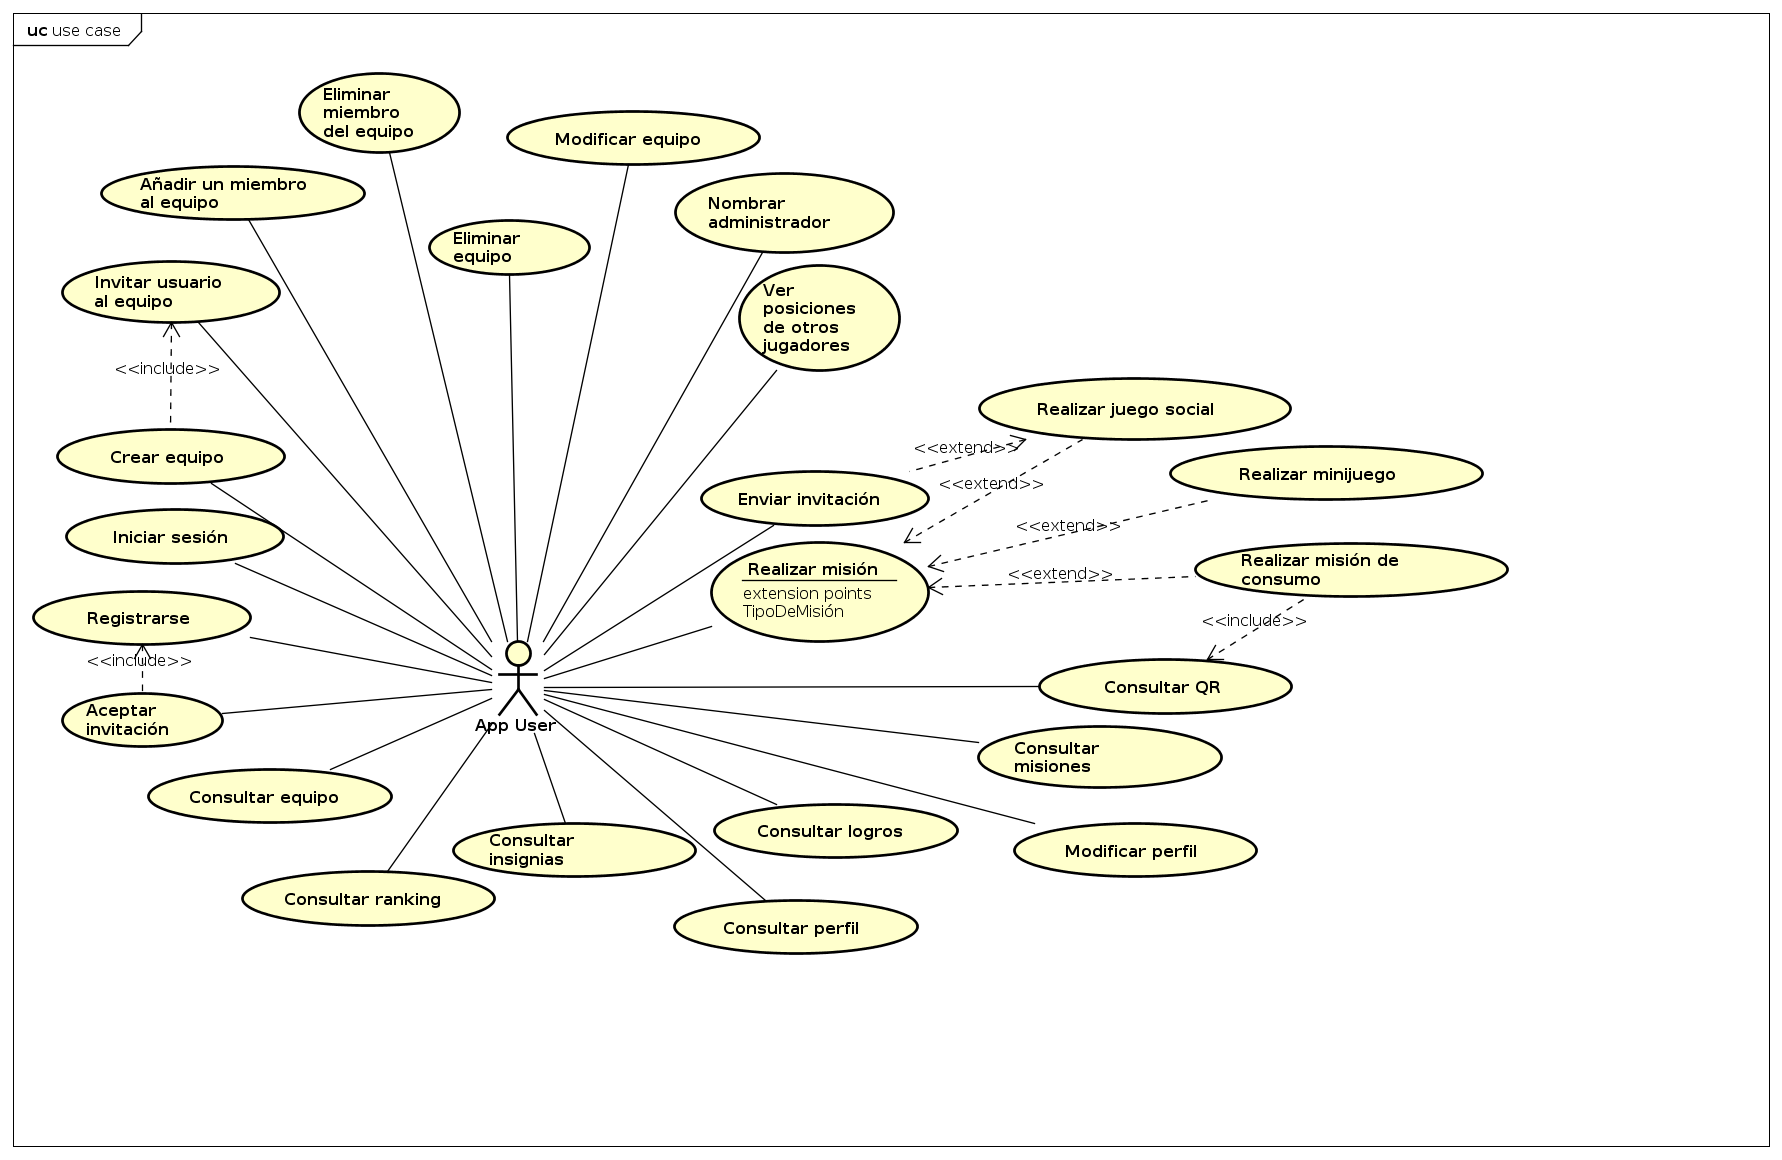
\includegraphics[angle=90,scale=0.5]{images/usecase.png}
\caption{Diagrama de casos de uso}
\end{center}
\end{figure}

\subsubsection{Actores}

Se identifican los siguientes actores:

\begin{itemize}
\item \textbf{Admin de grupo:} Es el actor encargado de administrar los grupos en los que tuviera este rol.
\item \textbf{App user:} Es el actor base de Route66App, en su parte de aplicación móvil.
\end{itemize}

\newcounter{usecase}\stepcounter{usecase}

\begin{usecase}
  \addheading{\textbf{CU\arabic{usecase}}}{Añadir un miembro al equipo} 
  \addrow{Actor}{Admin Grupo}
  \addrow{Precondiciones}{El usuario ha iniciado sesión en el sistema.}
  \addrow{Postcondiciones}{Ninguna.}
  \addrow{Flujo principal}{
  		\begin{enumerate}
  		\item El usuario selecciona “Añadir un miembro al equipo". %1
        \item El sistema muestra al usuario el listado de equipos. %2
        \item El usuario selecciona un equipo de la lista. %3
        \item El sistema pide al usuario el identificador del usuario que desea agregar al equipo. %4%
        \item El usuario introduce el identificador del usuario. %5
        \item El sistema agrega al usuario al equipo. %6
  		\end{enumerate}
  }
  \addrow{Flujos alternativos}{
  		\begin{itemize}
  		\item 1a 3a 5a El usuario cancela la operación. En este caso el caso de uso termina y queda sin efecto.
  		\item 2a El sistema no encuentra ningún equipo administrado por el usuario. En ese caso, se muestra un mensaje y el caso de uso queda sin efecto.
  		\item 5b El identificador de usuario no pertenece a ningún usuario de la aplicación. En este caso, se muestra un mensaje alertándolo y se vuelve al paso 4.
  		\end{itemize}
  }
\end{usecase}\\\stepcounter{usecase}


\begin{usecase}
  \addheading{\textbf{CU\arabic{usecase}}}{Modificar equipo} 
  \addrow{Actor}{Admin Grupo}
  \addrow{Precondiciones}{El usuario ha iniciado sesión en el sistema.}
  \addrow{Postcondiciones}{Ninguna.}
  \addrow{Flujo principal}{
  		\begin{enumerate}
  		\item El usuario selecciona “Gestionar un equipo". %1
        \item El sistema muestra al usuario el listado de equipos. %2
        \item El usuario selecciona un equipo de la lista. %3
        \item El sistema muestra el conjunto de parámetros de configuración del grupo, así como el valor de los mismos. %4
        \item El usuario elige un parámetro y lo modifica. %5
        \item El sistema actualiza la configuración del grupo. %6
  		\end{enumerate}
  }
  \addrow{Flujos alternativos}{
  		\begin{itemize}
  		\item 1a 3a 5a El usuario cancela la operación. En este caso el caso de uso termina y queda sin efecto.
  		\item 2a El sistema no encuentra ningún equipo administrado por el usuario. En ese caso, se muestra un mensaje y el caso de uso queda sin efecto.
  		\item 6a El parámetro introducido por el usuario no es válido (porque se ha introducido en un formato incorrecto). En ese caso, se notifica al usuario y se vuelve al paso 5.
  		\end{itemize}
  }
\end{usecase}\\\stepcounter{usecase}

\begin{usecase}
  \addheading{\textbf{CU\arabic{usecase}}}{Realizar misión} 
  \addrow{Actor}{App user}
  \addrow{Precondiciones}{El usuario ha iniciado sesión en el sistema.}
  \addrow{Postcondiciones}{Ninguna.}
  \addrow{Flujo principal}{
  		\begin{enumerate}
  		\item El usuario elige “Realizar misión". %1
  		\item El sistema muestra al usuario el conjunto de niveles con los que cuenta la aplicación. %2
  		\item El usuario escoge un nivel. %3
  		\item El sistema muestra al usuario las misiones de ese nivel. %4.
  		\item El usuario escoge la misión que desea realizar %5.
  		\item El sistema muestra al usuario la acción (juego, compartir por redes sociales, etcétera) que debe realizar para poder completar la misión. %6
  		\item El usuario completa la misión %7
  		\item El sistema actualiza la información, guardando que el usuario ha completado la misión. %8
  		\end{enumerate}
  }
  \addrow{Flujos alternativos}{
  		\begin{itemize}
  		\item 1a 3a 5a 7a El usuario cancela la operación. En este caso el caso de uso termina y queda sin efecto.
        \item 3b El usuario no selecciona el nivel que le corresponde completar (el nivel más bajo al que le falte por completar misiones). En ese caso, el sistema muestra un mensaje y vuelve al paso 2.
        \item 7b El usuario no completa la misión. En ese caso, se pregunta al usuario si desea volver a intentar
  		\end{itemize}
  }
\end{usecase}\\\stepcounter{usecase}

\begin{usecase}
  \addheading{\textbf{CU\arabic{usecase}}}{Realizar misión de consumo mínimo} 
  \addrow{Actor}{App user}
  \addrow{Precondiciones}{El usuario ha iniciado sesión en el sistema.}
  \addrow{Postcondiciones}{Ninguna.}
  \addmulrow{Flujo principal}{
  		\item User selects \ldots
        \item System demands \ldots
  }
  \addmulrow{Flujos alternativos}{
  		\item User selects \ldots
        \item System demands \ldots
  }
\end{usecase}\\\stepcounter{usecase}

\begin{usecase}
  \addheading{\textbf{CU\arabic{usecase}}}{Realizar minijuego.} 
  \addrow{Actor}{App user}
  \addrow{Precondiciones}{El usuario ha iniciado sesión en el sistema.}
  \addrow{Postcondiciones}{Ninguna.}
  \addmulrow{Flujo principal}{
  		\item User selects \ldots
        \item System demands \ldots
  }
  \addmulrow{Flujos alternativos}{
  		\item User selects \ldots
        \item System demands \ldots
  }
\end{usecase}\\\stepcounter{usecase}

\begin{usecase}
  \addheading{\textbf{CU\arabic{usecase}}}{Realizar juego social.} 
  \addrow{Actor}{App user}
  \addrow{Precondiciones}{El usuario ha iniciado sesión en el sistema.}
  \addrow{Postcondiciones}{Ninguna.}
  \addmulrow{Flujo principal}{
  		\item User selects \ldots
        \item System demands \ldots
  }
  \addmulrow{Flujos alternativos}{
  		\item User selects \ldots
        \item System demands \ldots
  }
\end{usecase}\\\stepcounter{usecase}

\begin{usecase}
  \addheading{\textbf{CU\arabic{usecase}}}{Consultar misiones} 
  \addrow{Actor}{App user}
  \addrow{Precondiciones}{El usuario ha iniciado sesión en el sistema.}
  \addrow{Postcondiciones}{Ninguna.}
  \addrow{Flujo principal}{
  		\begin{enumerate}
  		\item El usuario elige “Consultar misiones". %1
  		\item El sistema muestra al usuario el listado de niveles, destacando aquellos niveles que ya haya completado y marcando de una forma especial aquel nivel en el que se encuentre el usuario (que tenga misiones sin completar). %2
  		\item El usuario selecciona un nivel. %3
  		\item El sistema muestra al usuario las distintas misiones que conforman el nivel, destacando aquellas que hayan sido resueltas con anterioridad. %4
  		\end{enumerate}
  }
  \addrow{Flujos alternativos}{
  		\begin{itemize}
  		\item 3a. El usuario cancela la operación. En este caso el caso de uso termina y queda sin efecto.
  		\item 3b. El usuario ha seleccionado un nivel superior a aquel en el que se encuentra el usuario. En este caso, se muestra un mensaje al usuario y se vuelve al paso 2.
  		\end{itemize}
  }
\end{usecase}\\\stepcounter{usecase}

\begin{usecase}
  \addheading{\textbf{CU\arabic{usecase}}}{Modificar perfil} 
  \addrow{Actor}{App user}
  \addrow{Precondiciones}{El usuario ha iniciado sesión en el sistema.}
  \addrow{Postcondiciones}{Ninguna.}
  \addrow{Flujo principal}{
  		\begin{enumerate}
  		\item El usuario elige “Modificar perfil". %1
  		\item El sistema muestra al usuario el conjunto de parámetros que puede modificar y los valores que tiene asociados. %2
  		\item El usuario elige un parámetro y lo modifica. %3
  		\item El sistema actualiza el nuevo valor. %4
  		\end{enumerate}
  }
  \addrow{Flujos alternativos}{
  		\begin{itemize}
  		\item 1a 3a El usuario cancela la operación. En este caso el caso de uso termina y queda sin efecto.
  		\item 4a El parámetro introducido por el usuario no es válido (porque se ha introducido en un formato incorrecto). En ese caso, se notifica al usuario y se vuelve al paso 5.
  		\end{itemize}
  		}
\end{usecase}\\\stepcounter{usecase}

\begin{usecase}
  \addheading{\textbf{CU\arabic{usecase}}}{Consultar perfil} 
  \addrow{Actor}{App user}
  \addrow{Precondiciones}{El usuario ha iniciado sesión en el sistema.}
  \addrow{Postcondiciones}{Ninguna.}
  \addrow{Flujo principal}{
  		\begin{enumerate}
  		\item El usuario elige “Consultar perfil".
  		\item El sistema muestra al usuario su perfil, incluidos aquellos detalles como sus  “porcentajes de compromiso“ con la aplicación. (Ver página \pageref{rfcompromiso}).
  		\end{enumerate}
  }
\end{usecase}\\\stepcounter{usecase}

\begin{usecase}
  \addheading{\textbf{CU\arabic{usecase}}}{Consultar logros} 
  \addrow{Actor}{App user}
  \addrow{Precondiciones}{El usuario ha iniciado sesión en el sistema.}
  \addrow{Postcondiciones}{Ninguna.}
  \addmulrow{Flujo principal}{
  		\item User selects \ldots
        \item System demands \ldots
  }
  \addmulrow{Flujos alternativos}{
  		\item User selects \ldots
        \item System demands \ldots
  }
\end{usecase}\\\stepcounter{usecase}

\begin{usecase}
  \addheading{\textbf{CU\arabic{usecase}}}{Consultar insignias} 
  \addrow{Actor}{App user}
  \addrow{Precondiciones}{El usuario ha iniciado sesión en el sistema.}
  \addrow{Postcondiciones}{Ninguna.}
  \addmulrow{Flujo principal}{
  		\item User selects \ldots
        \item System demands \ldots
  }
  \addmulrow{Flujos alternativos}{
  		\item User selects \ldots
        \item System demands \ldots
  }
\end{usecase}\\\stepcounter{usecase}

\begin{usecase}
  \addheading{\textbf{CU\arabic{usecase}}}{Consultar código QR} 
  \addrow{Actor}{App user}
  \addrow{Precondiciones}{El usuario ha iniciado sesión en el sistema.}
  \addrow{Postcondiciones}{Ninguna.}
  \addmulrow{Flujo principal}{
  		\item User selects \ldots
        \item System demands \ldots
  }
  \addmulrow{Flujos alternativos}{
  		\item User selects \ldots
        \item System demands \ldots
  }
\end{usecase}\\\stepcounter{usecase}

\begin{usecase}
  \addheading{\textbf{CU\arabic{usecase}}}{Consultar ranking} 
  \addrow{Actor}{App user}
  \addrow{Precondiciones}{El usuario ha iniciado sesión en el sistema.}
  \addrow{Postcondiciones}{Ninguna.}
  \addmulrow{Flujo principal}{
  		\item User selects \ldots
        \item System demands \ldots
  }
  \addmulrow{Flujos alternativos}{
  		\item User selects \ldots
        \item System demands \ldots
  }
\end{usecase}\\\stepcounter{usecase}

\begin{usecase}
  \addheading{\textbf{CU\arabic{usecase}}}{Consultar equipo} 
  \addrow{Actor}{App user}
  \addrow{Precondiciones}{El usuario ha iniciado sesión en el sistema.}
  \addrow{Postcondiciones}{Ninguna.}
  \addmulrow{Flujo principal}{
  		\item User selects \ldots
        \item System demands \ldots
  }
  \addmulrow{Flujos alternativos}{
  		\item User selects \ldots
        \item System demands \ldots
  }
\end{usecase}\\\stepcounter{usecase}

\begin{usecase}
  \addheading{\textbf{CU\arabic{usecase}}}{Crear equipo} 
  \addrow{Actor}{App user}
  \addrow{Precondiciones}{El usuario ha iniciado sesión en el sistema.}
  \addrow{Postcondiciones}{Ninguna.}
  \addmulrow{Flujo principal}{
  		\item User selects \ldots
        \item System demands \ldots
  }
  \addmulrow{Flujos alternativos}{
  		\item User selects \ldots
        \item System demands \ldots
  }
\end{usecase}\\\stepcounter{usecase}

\begin{usecase}
  \addheading{\textbf{CU\arabic{usecase}}}{Registrarse} 
  \addrow{Actor}{App user}
  \addrow{Precondiciones}{Ninguna.}
  \addrow{Postcondiciones}{Ninguna.}
  \addmulrow{Flujo principal}{
  		\item User selects \ldots
        \item System demands \ldots
  }
  \addmulrow{Flujos alternativos}{
  		\item User selects \ldots
        \item System demands \ldots
  }
\end{usecase}\\\stepcounter{usecase}

\begin{usecase}
  \addheading{\textbf{CU\arabic{usecase}}}{Aceptar invitación.} 
  \addrow{Actor}{App user}
  \addrow{Precondiciones}{Ninguna.}
  \addrow{Postcondiciones}{Ninguna.}
  \addmulrow{Flujo principal}{
  		\item User selects \ldots
        \item System demands \ldots
  }
  \addmulrow{Flujos alternativos}{
  		\item User selects \ldots
        \item System demands \ldots
  }
\end{usecase}\\\stepcounter{usecase}

\begin{usecase}
  \addheading{\textbf{CU\arabic{usecase}}}{Enviar invitación} 
  \addrow{Actor}{App user}
  \addrow{Precondiciones}{El usuario ha iniciado sesión en el sistema.}
  \addrow{Postcondiciones}{Ninguna.}
  \addmulrow{Flujo principal}{
  		\item User selects \ldots
        \item System demands \ldots
  }
  \addmulrow{Flujos alternativos}{
  		\item User selects \ldots
        \item System demands \ldots
  }
\end{usecase}\\\stepcounter{usecase}

\begin{usecase}
  \addheading{\textbf{CU\arabic{usecase}}}{Iniciar sesión} 
  \addrow{Actor}{App user}
  \addrow{Precondiciones}{El usuario ha iniciado sesión en el sistema.}
  \addrow{Postcondiciones}{Ninguna.}
  \addmulrow{Flujo principal}{
  		\item User selects \ldots
        \item System demands \ldots
  }
  \addmulrow{Flujos alternativos}{
  		\item User selects \ldots
        \item System demands \ldots
  }
\end{usecase}\\\stepcounter{usecase}

\subsection{Modelo de dominio}

\begin{figure}[H]
\begin{center}
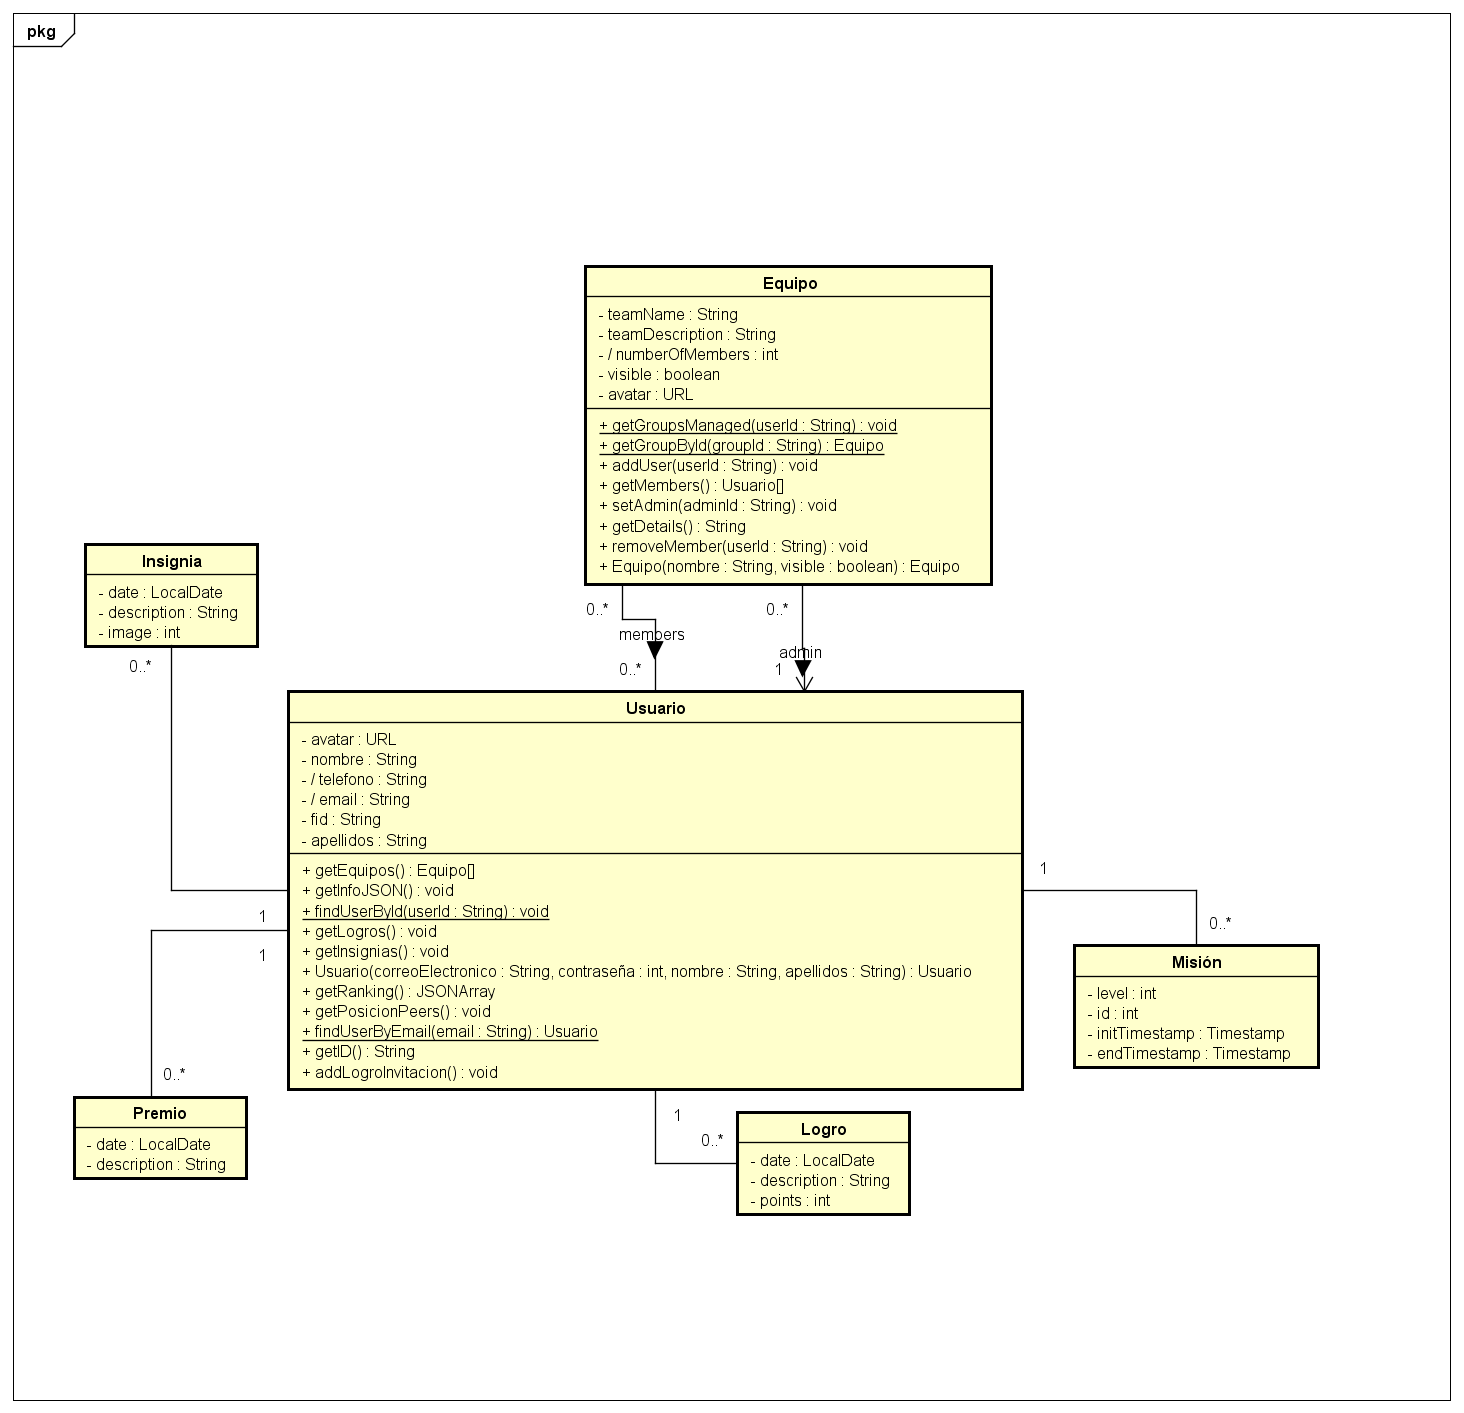
\includegraphics[angle=90,scale=0.5]{images/clases.png}
\caption{Modelo de dominio}
\end{center}
\end{figure}

\subsection{Diagrama de paquetes}
\section{Diseño}
\subsection{Arquitectura}
\subsection{Patrones utilizados}
\subsection{Esquema de la base de datos}
\subsection{Diagramas de secuencia}
\section{Implementación}
\section{Pruebas}

\chapter{Parte IV: Conclusiones y trabajo futuro.}
\section{Conclusiones}
\section{Trabajo futuro}
\chapter{Webgrafía y Bibliografía}
\begin{thebibliography}{a} 
\section{Webgrafía}

\bibitem{iebschoolGami} \textsc{Marc Rodríguez. IEBS Comunidad} \textit{La ludificación como fenómeno social y herramienta global}, Fecha de última visita: 6 de Noviembre de 2017 \url{http://comunidad.iebschool.com/pedrolopezugarte/2015/11/20/la-gamificacion-como-fenomeno-social-y-herramienta-global/}.  

\bibitem{confidencialcorreosgami} \textsc{María Benito} \textit{Gamificación o cómo lograr que los empleados hagan un trabajo extra gratis}, Fecha de última visita: 6 de Noviembre de 2017 \url{https://www.elconfidencial.com/empresas/2014-04-27/gamificacion-o-como-lograr-que-los-empleados-hagan-un-trabajo-extra-gratis_121168/}. 

\bibitem{accentureGami} \textsc{Accenture} \textit{Why gamification is serious business}, Fecha de última visita: 6 de Noviembre de 2017 \url{https://www.accenture.com/us-en/insight-outlook-why-gamification-is-serious-business}.  

\bibitem{bbvag} \textsc{Alejandro. Omnium Games.} \textit{BBVA Game: El mayor caso de éxito de la ludificación en España.}, Fecha de última visita: 21 de Noviembre de 2017 \url{http://omniumgames.com/bbva-game-el-mayor-caso-de-exito-de-la-gamificacion-en-espana/}.  

\bibitem{iebsctj} \textsc{Ferran Altarriba Bertran. IEBS School} \textit{Tipos de jugadores en Gamification: teoría Bartle}. Fecha de última visita: 6 de Noviembre de 2017, \url{http://www.iebschool.com/blog/tipos-jugadores-gamification-2-innovacion/}.  

\bibitem{mcdo} \textsc{McDonalds},\textit{Aplicación móvil McDonalds para Android} \url{https://play.google.com/store/apps/details?id=com.mcdonalds.android}


\bibitem{burgerk} \textsc{Burger King},\textit{Aplicación móvil Burger King para Android} \url{https://play.google.com/store/apps/details?id=es.burgerking.android}

\bibitem{kfcapp} \textsc{KFC},\textit{Aplicación móvil KFC para Android} \url{https://play.google.com/store/apps/details?id=es.kfc.spain}

\bibitem{vipsapp} \textsc{VIPS},\textit{Aplicación móvil VIPS para Android} \url{https://play.google.com/store/apps/details?id=com.clubvips.app}

\bibitem{pansapp} \textsc{Pans \& Company},\textit{Aplicación móvil Pans \& Company para Android} \url{https://play.google.com/store/apps/details?id=es.eatout.panscompany}

\bibitem{fostersh} \textsc{Foster's Hollywood},\textit{Aplicación móvil Foster's Hollywood para Android} \url{https://play.google.com/store/apps/details?id=com.zena.Fosters}

\bibitem{androidversiondist} \textsc{Android Developers Official Website},\textit{Dashboards. Platform Versions.} Fecha de última visita: 02 de Diciembre de 2017 \url{https://developer.android.com/about/dashboards/index.html}

\bibitem{infojobs2016} \textsc{Infojobs}. Estado del mercado laboral en España. Año 2016. pág 31. Fecha de última visita: 20/01/2018 \url{http://tueligesinfojobs.net/informe-anual-infojobs-2016.pdf} 

\bibitem{upedu} \textsc{Unified Process for Education. Universidad Politécnica de Montreal}. Fecha de última visita: 25/11/2017 \url{http://www.upedu.org/process/workers/wk_implm.htm}

\bibitem{monopolymcdo} \textsc{McDonalds}. Monopoly Ganador de McDonalds Fecha de última visita: 20/01/2018 \url{https://www.mcdonalds.es/sites/default/files/mcdonalds_lanza_su_nuevo_monopoly_ganador.pdf}

\bibitem{segsocialautonomos} \textsc{Infoautónomos. El Economista}. Tarifa plana de 50 \euro \hspace{0.1cm} para autónomos, jóvenes y mayores de 30. Fecha de última visita: 22/01/2018 \url{https://infoautonomos.eleconomista.es/seguridad-social/tarifa-plana-autonomos-50-euros-mayores-30-jovenes/}

\bibitem{pcuva} \textsc{Universidad de Valladolid. Parque Científico}. Oficinas del Parque Científico de la Universidad de Valladolid. Fecha de última visita: 22/01/2018 \url{http://www.parquecientificouva.es/Upload/ESPACIOS/CTTA/CTTA_FichaOficinas_Jun2013.pdf}



\section{Bibliografía}

\bibitem{cristinatfg} \textsc{Cristina Martínez Martínez} \textit{TFG “Estudio de ludificación en una empresa para mejorar la fidelización de los clientes”}. Curso 2016-2017. Grado en Organización Industrial. Universidad de Valladolid. 

\bibitem{anatfg} \textsc{Ana Ruiz Caballero} \textit{Trabajo de Fin de Grado “Estudio de la ludificación de una empresa para incentivar la motivación. "}. Curso 2015-2016. Grado en Organización Industrial. Universidad de Valladolid. 

\bibitem{pgpup} \textsc{De la Fuente Redondo, Pablo Lucio}. Departamento de Informática de la UVa, \textit{Apuntes de la asignatura Planificación y Gestión de Proyectos. Curso 2017-2018. Tema 3: Proceso Unificado}

\bibitem{pgptema2} \textsc{De la Fuente Redondo, Pablo Lucio}. Departamento de Informática de la UVa. Apuntes de la asignatura Planificación y Gestión de Proyectos. Curso 2017-2018. Tema 2: Planificación de Proyectos.


\end{thebibliography}

\chapter{Anexos}



\end{document}